%%%%%%%%%%%%%%%%%%%%%%%%%%%%%%%%%%%%%%
% corey_adams_thesis.tex
% Corey Adams
% 2016
%
% Using a custom style sheet, this is the main document for my thesis
%%%%%%%%%%%%%%%%%%%%%%%%%%%%%%%%%%%%%%

\documentclass[letterpaper,11pt]{yalephd}
% remove draft option for final printing.
% font size must be between 10pt-12pt.


\usepackage{geometry} % you need this for yalephd.cls to work.
\usepackage{graphicx} % you probably want the rest of these.
\usepackage{dcolumn}
\usepackage{bm}
\usepackage{amsmath}
\usepackage{amsfonts}
\usepackage{amssymb}
\usepackage{appendix}
\usepackage{comment}
\usepackage{cite}
\usepackage{notoccite}
\usepackage{xspace}
\usepackage{subcaption}
\usepackage[makeroom]{cancel}
\usepackage{adjustbox}

% This is a font, kind of similar to Times New Roman
\usepackage{mathptmx}

\usepackage{hyperref}
\hypersetup{
    colorlinks,
    citecolor=black,
    filecolor=black,
    linkcolor=black,
    urlcolor=black
}

%% command definitions
\newcommand{\lartpc}{\text{LAr-TPC}\xspace}
\newcommand{\lartpcs}{\text{LAr-TPCs}\xspace}
\newcommand{\uboone}{\text{MicroBooNE}\xspace}
\newcommand{\MB}{MiniBooNE\xspace}
\newcommand{\uB}{MicroBooNE\xspace}
\newcommand{\SB}{SciBooNE\xspace}
\newcommand{\sbnd}{SBND\xspace}
\newcommand{\icarus}{ICARUS-T600\xspace}
\newcommand{\nova}{\text{NO\ensuremath{\nu}A}\xspace}
\newcommand{\argoneut}{\text{ArgoNeuT}}

\newcommand{\numu}{\ensuremath{\nu_{\mu}}\xspace}
\newcommand{\nue}{\ensuremath{\nu_{e}}\xspace}
\newcommand{\nutau}{\ensuremath{\nu_{\tau}}\xspace}
\newcommand{\numubar}{\ensuremath{\bar\nu_{\mu}}\xspace}
\newcommand{\nuebar}{\ensuremath{\bar\nu_{e}}\xspace}
\newcommand{\nutaubar}{\ensuremath{\bar\nu_{\tau}}\xspace}
\newcommand{\nuone}{\ensuremath{\nu_{1}}\xspace}
\newcommand{\nutwo}{\ensuremath{\nu_{2}}\xspace}
\newcommand{\nuthree}{\ensuremath{\nu_{3}}\xspace}
\newcommand{\nufour}{\ensuremath{\nu_{4}}\xspace}
\newcommand{\nufive}{\ensuremath{\nu_{5}}\xspace}
\newcommand{\nualpha}{\ensuremath{\nu_{\alpha}}\xspace}
\newcommand{\nubeta}{\ensuremath{\nu_{\beta}}\xspace}
\newcommand{\pizero}{\ensuremath{\pi^{0}}\xspace}

\newcommand{\numunue}{\ensuremath{\numu \rightarrow \nue}\xspace}
\newcommand{\numunuebar}{\ensuremath{\bar{\nu}_{\mu} \rightarrow \bar{\nu}_{e}}\xspace}
\newcommand{\numunueboth}{\ensuremath{\overset{\text{\tiny (}-\text{\tiny )}}{\numu} \rightarrow \overset{\text{\tiny (}-\text{\tiny )}}{\nue}\xspace}}
\newcommand{\numudis}{\ensuremath{\numu \rightarrow \nu_{x}}\xspace}
\newcommand{\nuedis}{\ensuremath{\nue \rightarrow \nu_{x}}\xspace}
\newcommand{\numunumu}{\ensuremath{\numu \rightarrow \numu}\xspace}
\newcommand{\dmsq}{\ensuremath{\Delta m^2}\xspace}
\newcommand{\dmsqfourone}{\ensuremath{\Delta m^2_{41}}\xspace}
\newcommand{\sinth}{\ensuremath{\sin^22\theta}\xspace}
\newcommand{\Enu}{\ensuremath{E_{\nu}}\xspace}
\newcommand{\dcp}{\ensuremath{\delta_{\mathrm{CP}}}}
\newcommand{\lenu}{\ensuremath{L/E_{\nu}}\xspace}

\newcommand{\GeV}{\ensuremath{\mbox{GeV}}\xspace}
\newcommand{\MeV}{\ensuremath{\mbox{MeV}}\xspace}
\newcommand{\GeVc}{\ensuremath{\mbox{GeV}/c}\xspace}
\newcommand{\MeVc}{\ensuremath{\mbox{MeV}/c}\xspace}
\newcommand{\GeVcc}{\ensuremath{\mbox{GeV}/c^2}\xspace}
\newcommand{\eVsq}{\ensuremath{\mbox{eV}^2}\xspace}


% Bibliography stuff:
\bibliographystyle{abbrvunsrt}



\begin{document}



% This file contains all the stuff at the very beginning of the thesis: title page, abstract, title of contents, list of figures, etc...

% Need to define title before the abstract.
\title{Electron Neutrinos in Liquid Argon Time Projection Chambers}
\author{Corey Adams}
\advisor{Professor Bonnie Fleming}
\date{December, 2016} % usually not \today.

% All the stuff at the front of your thesis.
\frontmatter


\begin{abstract}

Electron neutrinos are at the center of the U.S. and international accelerator based neutrino program.  They are the flagship oscillation channel for DUNE, \uboone, and the Fermilab Short Baseline Neutrino Program.  Liquid argon time projection chambers are the forefront of neutrino detection technology, and the detector of choice for both short and long baseline neutrino oscillation experiments.

This work presents the first experimental observation and study of electron neutrinos in the 1-10 GeV range, the essential oscillation energy regime for the above experiments.  The systematic uncertainties for an electron neutrino appearance search for the Fermilab Short Baseline Neutrino Program are carefully quantified, and the characterization of separation between electrons and high energy photons is examined.

\end{abstract}

\maketitle

\makecopyright{2016} % change as needed.

\newpage \vspace*{8cm}
% Sets a PDF bookmark for the dedication
\pdfbookmark{Dedication}{dedication}
\thispagestyle{empty}
\begin{center}
  \Large \emph{For Shannon, \\ and my parents}
\end{center}

% This section describes what's happening in this thesis:




\tableofcontents
\listoffigures % remove this if you have no figures.
\listoftables % remove this if you have no tables.



\chapter{Acknowledgements} % this needs to be before \mainmatter.




% Starts proper arabic numbering of pages and chapters.
\mainmatter

\chapter{\label{chp:intro} Neutrino Physics}


Since its original inception in the 1930s, neutrino physics has developed into a robust field of high energy physics.  The neutrino was theorized in the 1930s by Wolfgang Pauli, rigorously incorporated into the theory of beta decay by Enrico Fermi \cite{Fermi}, and first detected in 1956 by Clyde Cowan and Frederick Reines \cite{Cowan:1992xc}.

Originally, the neutrino was postulated to preserve conservation of momentum in the theory of beta decay, where a nucleon such as a neutron is converted to a proton by emitting an electron and a neutrino:
\begin{equation}
\label{beta_decay}
n \rightarrow p^+ + e^- + \nuebar
\end{equation}

The reaction above is actually an example of a weak interaction happening at the quark level, where one of the neutron's down quarks converts to an up quark through the emission of a $W^-$.  Unfortunately, the neutrino is a very weakly interacting particle, so the direct observation of both the electron and the neutrino from a $\beta$ decay reaction was, and still is, impossible.  

For the detection of the neutrino, Cowan and Reines used a very similar reaction to beta decay, but instead of producing a neutrino this reaction absorbs a neutrino and emits a neutron and a positron:
\begin{equation}
\label{inverse_beta_decay}
p^+  + \nuebar \rightarrow e^- + n 
\end{equation}

Unlike neutrinos, neutrons and positrons are relatively easy to observe, so Cowan and Reines simply exposed a large sample of protons to a very large blast of neutrinos.  Practically, this meant building a detector near a high intensity source of neutrinos, which they did: they exposed large tanks of water to the neutrino flux of a nuclear reactor at the Savannah River plant, in Georgia.  The neutrinos coming to their detector (actually, {\em anti}-neutrinos) interacted with the protons and produced a neutron and a positron.  The positron was observed after it interacted by annihilating with an electron in the water tank, producing a pair of gamma particles.  The neutron was detected by it's capture on Cadmium, which was doped in the tank.  The neutron capture also produces a gamma, but it is delayed from the positron's gamma pair.  Cowan and Reines ultimately observed about three neutrinos per hour in their detector.  Conclusively, when the reactor was shut off, they no longer observed neutrinos. 

Since the first discovery of the neutrino, neutrinos and their interactions have played a central role in the development of the standard model of particle physics.  Pauli originally proposed only one neutrino, but not long after his prediction (and before the experimental evidence that confirmed it) other types of neutrinos were postulated.   Since then, 2 other types of neutrinos have been discovered, namely the muon and tau neutrinos \cite{PhysRevLett.9.36},\cite{Kodama:2000mp}. 

Conventionally, neutrinos are symbolized as $\nu_e, \nu_\mu,$ and $\nu_\tau$ corresponding to the 3 flavors of charged leptons.  The charged current interactions of these neutrinos, by exchanging a $W^\pm$ boson, produces an outgoing charged lepton of the same flavor as the incoming neutrino: \nue produces electrons, \nuebar produces anti-electrons, \numu produces muons, etc, such as in Equations~\ref{beta_decay} and \ref{inverse_beta_decay}.  However, neutrinos can also interact via neutral currents, where the outgoing lepton is {\em not} charged.  Instead, the neutrino exchanges a neutral $Z^0$ boson with the target material.  The first observed neutral current interaction is shown in Figure~\ref{fig:gargamelle_nc} \cite{Hasert:1973ff}.

\begin{figure}[htbp]
  \centering
  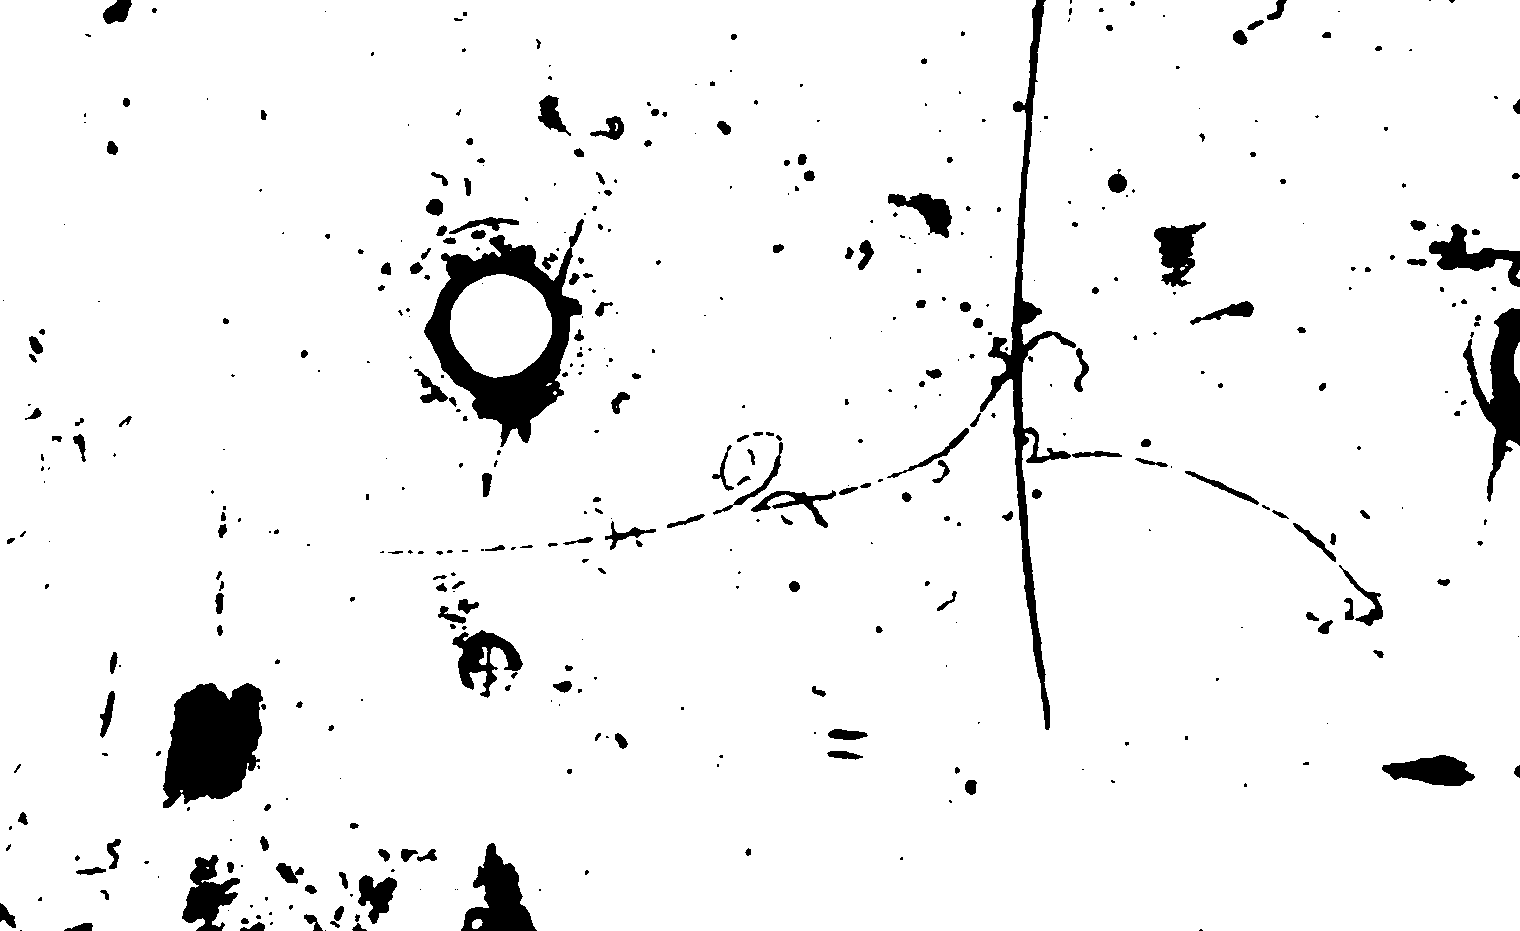
\includegraphics[width=0.95\textwidth]{intro_figures/gargamelle_nc.png}
  \caption[First Observed Neutral Current Neutrino Interaction]{The first observed neutral current neutrino interaction, seen by Gargamelle in 1973.}
  \label{fig:gargamelle_nc}
\end{figure}


Neutrino physics was dramatically altered with the discovery of neutrino oscillations, described below, which opens the door to measurements of CP Violation and possible sterile states of neutrinos.  Since the 1960s until the early 2000s, the field of neutrino physics had an unresolved anomaly known as the Solar Neutrino Problem.  Models of the interactions in the interior of the sun made a definite prediction for the number of electron-flavor neutrinos arriving at Earth \cite{Bahcall:2004pz}, based on well grounded theories of stellar fuel burning.  On the other hand, experiments sensitive to neutrinos observed a significant deficit as compared to predictions \cite{Davis:1968cp}.  It wasn't until the GALLEX/SAGE \cite{Hampel:1997fc, Abdurashitov:1998ne} experiments, along with the Super-Kamiokande experiment \cite{PhysRevLett.81.1562} and the Sudbury Neutrino Observatory \cite{Ahmad:2002jz}, that a solution to the Solar Neutrino Anomaly was found through the mechanism of oscillations: the sun did in fact produce the predicted rate of electron neutrinos, but experiments that were only sensitive to electron neutrinos were unable to detect the muon and tau neutrinos that were produced through the oscillation mechanism.  

The conclusive evidence for neutrino oscillations also implies that neutrinos are not, as was initially believed, massless particles.  However, neutrinos are known to be incredibly light weight, and cosmological constraints imply neutrinos have a summed mass (all three active flavors) of less than 0.23 eV \cite{Abazajian:2011dt, Ade:2013zuv}.  The exact mass of each type of neutrino is unknown still, though experiments are setting lower and lower bounds to directly constrain it \cite{BORNSCHEIN200514, Mertens:2014nha}.

One of the most exciting questions that may be addressed by studying neutrinos is CP violation.  Some theories predict that the current matter/anti-matter imbalance in the observable universe can be explained by CP violation by leptons, such as neutrinos \cite{Nunokawa:2007qh}.  This parameter is directly probable with neutrinos by measuring the difference in neutrino oscillations between neutrinos and anti-neutrinos, as described below.  In particular, the neutrino matter effect \cite{Wolfenstein:1977ue, Mikheev:1986gs} leads to a large observable effect of CP violation in electron neutrinos.

Another intriguing avenue of discovery in neutrino physics is the resolution of short baseline anomalies, which may hint towards the existence of sterile neutrinos.  Experiments have been proposed to probe these anomalies \cite{Antonello:2015lea, Ashenfelter:2015uxt}, and other existing experiments have found ways to investigate short baseline anomalies already \cite{TheIceCube:2016oqi, Adamson:2010wi, MINOS:2016viw, An:2014bik}.

Both for the case of CP violation and the resolution of short baseline anomalies, the detection and measurement of electron neutrinos crucial.  The most promising proposal to measure CP violation, DUNE \cite{Acciarri:2016ooe}, will look for the appearance of electron neutrinos in a primarily muon neutrino beam.  The Fermilab Short Baseline Neutrino Program (SBN Program) \cite{Antonello:2015lea} will similarly be searching for electron neutrinos in a primarily muon neutrino neutrino beam.  The first stage of the SBN Program, \uboone, is already running in Fermilab's Booster Neutrino Beam searching for low energy electron neutrinos.

Both DUNE and the SBN Program rely on high granularity detectors for their neutrino searches, the liquid argon time projection chamber (LArTPC, see Chapter~\ref{chp:lartpcs}).  However, at the time of the publication of this thesis, only one \lartpc in the world has ever observed electron neutrinos.  The ICARUS experiment includes an observation of two electron neutrinos at approximately 20 GeV \cite{Antonello:2013gut}.  On the other hand, the energy of interest to both DUNE and SBN is significantly lower, in the range of 1 GeV.  Therefore, the work presented in this thesis is the first observation of low energy electron neutrinos in a liquid argon time projection chamber.   

\section{Neutrino Sources}

Neutrinos, despite their weak interaction cross section and difficulty to observe, are actually incredibly common on Earth - more than a trillion neutrinos pass through an average sized human hand every second.  By far the most powerful nearby source of neutrinos is from the Sun, produced predominantly in proton-proton fusion.  But, more powerful (and more exotic) sources of neutrinos are known to exist, such as supernova \cite{Dadykin:1987ek, Hirata:1988ad}.  Terrestrially, neutrinos are produced in the geothermal reactions of the Earth's core, and there is large flux of ``atmospheric'' neutrinos produced by the interactions of cosmic particles in the upper atmosphere.  As radioactive elements decay through weak interactions, radioactive material emits neutrinos as well - in fact this can be a quite useful source for calibration of neutrino experiments.

There are also artificial sources of neutrinos, most commonly nuclear reactors.  Though they are less powerful than the Sun, neutrino experiments can get significantly closer to a nuclear reactor than to the Sun, and the local neutrino flux can be quite high.  The most sophisticated artificial source of neutrinos comes from the neutrinos beams produced at accelerator complexes such as Fermilab, CERN, and J-PARC.  Artificial neutrino beams can provide a high intensity source of neutrinos over a large range of energies, and offer many other benefits as well.  

A detailed understanding of the source of neutrinos is vital to the success of every neutrino experiment, and Chapter~\ref{chp:beams} explores neutrino beams in more detail.

% \subsection{Solar Neutrinos}

% \subsection{Atmospheric Neutrinos}

% \subsection{Supernova Neutrinos}

% \subsection{Radioactive Sources}

% \subsection{Reactor Neutrinos}

% \subsection{Neutrino Beams}

\section{Neutrino Oscillations}

Neutrino oscillations \cite{Bilenky:1978nj, Maki:1962mu, Langacker:1988up} are the foundation and the starting point for modern neutrino experiments exploring CP violation and short baseline anomalies, and can be used to probe the mass hierarchy of the neutrinos.  As such, they are fundamentally important to neutrino experiments, so a description of the theory of neutrino oscillations and the experimental evidence is presented here.

\subsection{Neutrino Oscillations - Theory}


Neutrinos, when produced through electro-weak interactions, are produced in flavor eigenstates.  To date, there are known to be three flavors of neutrinos: \nue, \numu, and \nutau.  Each of these neutrinos, as suggested by their name, corresponds to a charged lepton.  The conservation of lepton flavor, in electro-weak interactions, dictates that the number of leptons of a particular flavor is conserved during an interaction.  As an example, the decay of a muon to an electron would violate lepton flavor conservation if not for the presence of neutrinos:

\begin{equation}
\mu^- \rightarrow e^- + \bar{\nu}_e + \nu_\mu
\end{equation}

Lepton flavor violation is not, however, a law of nature.  The most striking evidence for the violation of lepton flavor conservation is neutrino oscillations, though there are hints and proposals that lepton flavor could be violated by charged leptons as well \cite{Bartoszek:2014mya}.  For neutrino oscillations, the violation of lepton flavor is a direct result of the fact that neutrinos in the lepton eigenstates are a superposition of the mass eigenstates of neutrinos:

\begin{equation}
\nu_e = \alpha \nu_1 + \beta \nu_2 + \gamma \nu_3
\end{equation}

where the numerical neutrino states represent the neutrinos with a well defined mass.  It should be noted, from a historical perspective, that in fact neutrinos were originally considered to be zero-mass in the Standard Model.  The discovery of neutrino oscillations instead provided definitive evidence that neutrinos {\bf do} have mass.  From a modern perspective, however, the evidence for neutrino masses is overwhelming.  The interesting phenomenon, then, arise from the fact that neutrinos produce in lepton flavor states do not stay stably in those states.  

The most common way to mathematically describe neutrino oscillations is through the Pontecorvo-Maki-Nakagawa-Sakata matrix \cite{Maki:1962mu, Bilenky:1978nj}, or PMNS matrix:

\begin{equation}
  \left(
  \begin{array}{c}
    \nu_e \\
    \nu_\mu \\
    \nu_\tau \\
  \end{array}
  \right)
  =
  \left(
  \begin{array}{ccc}
    U_{e1} & U_{e2} & U_{e3}  \\
    U_{\mu1} & U_{\mu2} & U_{\mu3}  \\
    U_{\tau1} & U_{\tau2} & U_{\tau3}  \\
  \end{array} 
  \right)
  \left(
  \begin{array}{c}
    \nu_1 \\
    \nu_2 \\
    \nu_3 \\
  \end{array}
  \right)
\end{equation}

In this matrix, under the standard assumptions of neutrino oscillations, the rows and columns are normalize such that the matrix is  unitary: $\sum_{i=1}^3 | U_{\alpha i} | ^2 = 1$, and similarly for the columns.  It's very common for the PMNS matrix to be parameterize in terms of mixing angles: 

\begin{align}
  \left(
  \begin{array}{ccc}
    U_{e1} & U_{e2} & U_{e3}  \\
    U_{\mu1} & U_{\mu2} & U_{\mu3}  \\
    U_{\tau1} & U_{\tau2} & U_{\tau3}  \\
  \end{array} 
  \right)
  = 
  \left(
  \begin{array}{ccc}
    1 & 0 & 0  \\
    0 & \text{cos}\theta_{23} & \text{sin}\theta_{23}  \\
    0 & -\text{sin}\theta_{23} & \text{cos}\theta_{23}  \\
  \end{array} 
  \right)
  &\times \\
  \left(
  \begin{array}{ccc}
     \text{cos}\theta_{13} & 0 & \text{sin}\theta_{13} e^{ - i \delta_{CP}}  \\
     0 & 1 & 0  \\
     -\text{sin}\theta_{13} e^{i \delta_{CP}} & 0 & \text{cos}\theta_{13}  \\
  \end{array} 
  \right)
  &\times \\
  \left(
  \begin{array}{ccc}
    \text{cos}\theta_{12} & \text{sin}\theta_{23} & 0  \\
    - \text{sin}\theta_{23} & \text{cos}\theta_{12} & 0 \\
    0 & 0 & 1  \\
  \end{array} 
  \right)
\end{align}

The value of this expansion is that the individual mixing angles are observable with different experimental setups.  The additional phase, $\delta_{CP}$, is needed if neutrinos violate Charge-Parity symmetry.  Some theories suggest that neutrino violation of CP symmetry is responsible for the matter/anti-matter asymmetry in the Universe (see Section~\ref{sec:future_experiments}).

In general, an experiment probing neutrino oscillations will start with an ensemble of neutrinos prepared in a particular flavor state $\nu_\alpha$:
\begin{equation*}
\nu_\alpha = U_{\alpha 1} \nu_1 + U_{\alpha 2} \nu_2 + U_{\alpha 3} \nu_3
\end{equation*}

The state of the neutrino $\nu_\alpha$ evolves according to the standard time evolution operator, and so at a later time the neutrino state is  
\begin{equation*}
\nu_\alpha (t) = U_{\alpha 1} \nu_1(t) + U_{\alpha 2} \nu_2(t) + U_{\alpha 3} \nu_3(t)
\end{equation*}

where $\nu_{j}(t) = e^{-i ( E_j t - \vec{p} \dot \vec{x})} \nu_j (t)$, using the plane wave solution for the neutrinos.  Since each neutrino has a different mass, the three components of a neutrino flavor state become out of phase as time passes.  Since the neutrino masses are known to be very small, and the neutrinos detected in experiments are typically energies of MeV or higher, all observed neutrinos are ultra-relativistic.  So, the energy expression in the time evolution of the neutrino flavor state can be simplified with $E_j \approx E + \frac{m_j^2}{2E}$.  Therefore, the probability that a neutrino that started in state $\alpha$ will be observed in state $\beta$ at a later time $t$ is:

\begin{equation*}
P_{\alpha\rightarrow\beta} = \left|\braket{\nu_\alpha(t) | \nu_\beta}\right|^2 = \left|\sum_i U_{i\alpha} U_{i\beta} e^{-i t \frac{m_j^2 }{ 2 E}}\right|^2
\end{equation*}

Of course, since neutrinos are ultra-relativistic it is not possible to observe them at a later time in the same location.  Instead, neutrino oscillations searches observe the neutrinos at a distance away from the source.  Assuming the neutrinos travel at the speed of light, so that $L = c t$ (and typically setting c = 1), the useful oscillation probability expression for neutrino experiments is 

\begin{equation*}
P_{\alpha\rightarrow\beta} = \left|\sum_i U_{i\alpha} U_{i\beta} e^{-i m_j^2 \frac{L}{2E}}\right|^2
\end{equation*}

For the case of oscillation between two types of neutrinos, the oscillation probability is often expressed as

\begin{equation}
P_{\alpha\rightarrow\beta} = \text{sin}^2(2\theta)\text{sin}^2\left( \frac{\Delta m^2 L}{4 E} \right)
\end{equation}

As seen in the next section, the sinusoidal characteristic of oscillations is apparent when the neutrinos are presented as a function of $L/E$.

\subsection{Neutrino Oscillations - Experimental Evidence}

Neutrino oscillations have a compelling record of experimental evidence in their favor.  This section provides a brief overview of some of the notable oscillation experiments to date.  A much more complete summary of neutrino oscillations, both theory and experimental evidence, is available from the Particle Data Group \cite{Agashe:2014kda}.

\subsubsection{Solar Neutrino Problem}

The first experimental hint of neutrino oscillations came, retrospectively, with the ``Solar Neutrino Problem.''  The standard Solar model makes a definite prediction for the number of neutrinos produced by the sun \cite{Bahcall:2004pz}, while the observation of Ray Davis and John Bahcall at the Homestake experiment observed only approximately one third of the neutrinos they expected from the Sun.  This observation was subsequently reproduced and confirmed by a number of experiments \cite{Hampel:1998xg, Fukuda:1996sz, Gavrin:2005ks, Anselmann:1992um, Altmann:2005ix, Fukuda:2002pe, Ahmad:2001an, Ahmad:2002jz}.

The many neutrino detectors observing the solar neutrinos produced different measurements of their observed flux, compared to predictions from standard solar models - see Figure~\ref{fig:solar_neutrino_deficit}.  Each experiment, however, observes a different deficit of neutrinos.  However, the experiments searching for solar neutrinos had different minimum thresholds for detection, and the solar neutrino flux is not constant with energy (Figure~\ref{fig:solar_neutrino_flux}).  This strongly implied that the resolution of the Solar Neutrino Problem needed to account for a dependence on neutrino energy, consistent with neutrino oscillations.  Further, the evidence was very strong that the neutrino oscillations in the Sun were affected by the interactions of neutrinos with matter, know as the Mikheev-Smirnov-Wolfenstien (MSW) effect \cite{Wolfenstein:1977ue,Mikheev:1986gs}.

\begin{figure}[htbp]
  \centering
  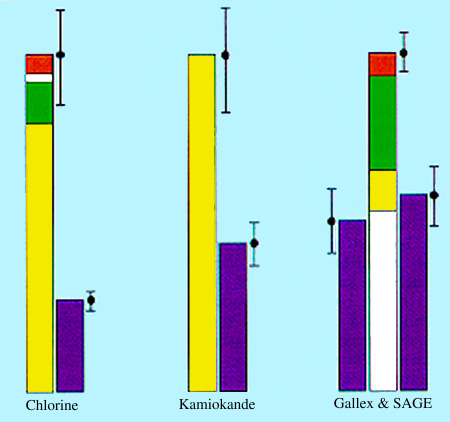
\includegraphics[width=0.45\textwidth]{intro_figures/solar_neutrino_deficit.png}
  \caption[Solar Neutrino Deficit]{Solar neutrino deficit for the different detectors/materials.  Figure from \cite{solar_neutrino_image}.}
  \label{fig:solar_neutrino_deficit}
\end{figure}

\begin{figure}[htbp]
  \centering
  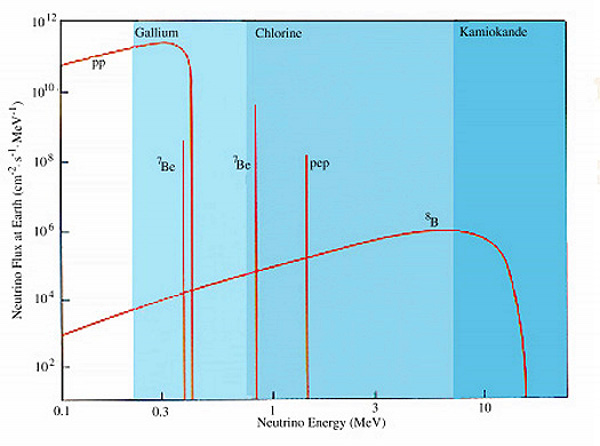
\includegraphics[width=0.65\textwidth]{intro_figures/solar_neutrino_flux.png}
  \caption[Solar Neutrino Flux]{Solar neutrino flux, and the relevant region for the different detectors/materials.  Figure from \cite{solar_neutrino_image}.}
  \label{fig:solar_neutrino_flux}
\end{figure}

Eventually, with the results of experiments such as Super Kamiokande and and SNO, the squared mass separation required to explain the solar neutrino deficit in terms of oscillations was measured as $m_{solar} = 7.5 \times 10^{-5} eV^2$.  This measurement was later confirmed by the KamLAND experiment \cite{Eguchi:2002dm, Araki:2004mb}, who also were able to demonstrate experimentally the sinusoidal dependence of neutrino oscillations, in Figure~\ref{fig:kamland}.  Combined with solar neutrino data, the KamLAND results \cite{Abe:2008aa,Gando:2010aa} indicated that the solar neutrino mass splitting, now understood to be $\Delta m^2_{12}$, is $\Delta m^2{12} = 7.5^{+0.19}_{-0.20} \times 10^{-5} eV^2$, and the oscillation mixing angle is given as $\text{tan}^2(\theta_{12}) = 0.452^{+0.035}_{-0.033}$.

\begin{figure}[htbp]
  \centering
  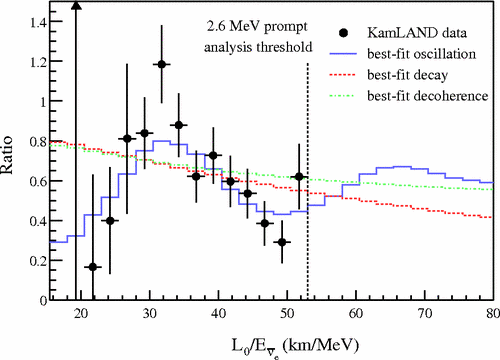
\includegraphics[width=0.45\textwidth]{intro_figures/kamland.png}
  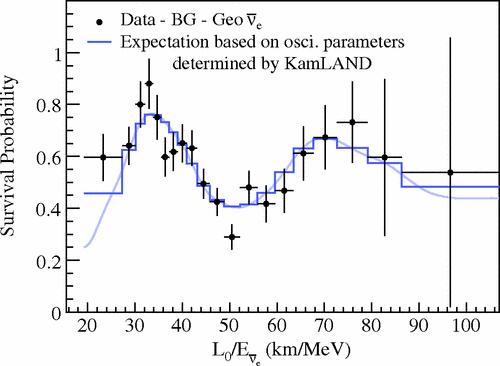
\includegraphics[width=0.45\textwidth]{intro_figures/kamland_highstats.png}
  \caption[KamLAND Oscillation Results]{(Left) Initial oscillation spectrum from KamLAND. (Right) Higher statistics results from KamLAND.  The data are plotted with L=180km, and the data agree well with the best fit oscillation hypothesis. Figures from \cite{Araki:2004mb,Abe:2008aa}.}
  \label{fig:kamland}.
\end{figure}

The resolution of the solar neutrino anomaly set off a cascade of neutrino oscillation searches, including the search for oscillations outside of the solar neutrino regime.  The observation of atmospheric oscillations, in fact, was historically the first direct evidence of neutrino oscillations.

\subsubsection{Atmospheric Neutrinos}

Earth is continuously bombarded with particles in the upper atmosphere, producing (among other things) a flux of neutrinos primarily from the decay of pions and kaons \cite{Honda:2004yz, PhysRevD.70.023006, Plyaskin:2001ku}.  The atmospheric flux is often predicted as a function of zenith angle, and this allows neutrino oscillation experiments to study neutrinos over a very large range of distances: the shortest distances of travel from production are 10s of kilometers, directly above a detector, to $1.2 \times 10^4$ kilometers, from the opposite side of the Earth.  The atmospheric neutrino flux is composed of primarily of \numu, \numubar, \nue, and \nuebar neutrinos in approximately a 2:1 ratio for (\numu + \numubar) : (\nue + \nuebar) \cite{Agashe:2014kda}.

Compelling evidence for the oscillation of atmospheric muon neutrinos was presented by the Super-Kamiokande collaboration in 1998 \cite{PhysRevLett.81.1562}, shown in Figure~\ref{fig:super_k_oscillations}.  Because the Super-Kamiokande detector is unable to distinguish muons from anti-muons, there is no ability to sign select and the oscillation result is presented as a combined oscillation of muon neutrinos and anti-neutrinos.  Because of the distances involved and the energy range of the neutrinos, the solar neutrino mixing is not plausible as an explanation for the oscillation of atmospheric neutrinos.  In addition, the electron neutrino component of the flux is in general agreement with the observed data, assuming no oscillations.  Therefore, the explanation is that atmospheric muon neutrinos oscillate into tau neutrinos.  A subsequent study confirmed the statistical observation of tau neutrinos from atmospheric oscillations, though the tau neutrinos can not be identified on an event-by-event basis \cite{PhysRevLett.110.181802}.  The atmospheric neutrino oscillation suggests a mass splitting that is in the range of $10^{-3} eV^2$, significantly higher than the observed solar neutrino mass splitting.

\begin{figure}[htbp]
  \centering
  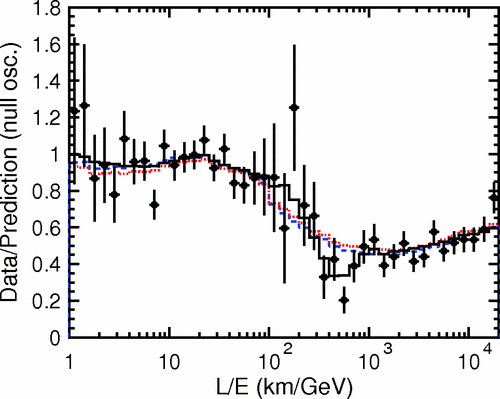
\includegraphics[width=0.65\textwidth]{intro_figures/superk_atmospheric_oscillation.png}
  \caption[Super-K Neutrino Oscillations]{Super-Kamiokande atmospheric neutrino oscillations, as a function of L/E.  L is calculated from the zenith angle of the detected neutrino. Figure from \cite{PhysRevLett.93.101801}.}
  \label{fig:super_k_oscillations}
\end{figure}

\subsubsection{On-axis Neutrino Beams: K2K and MINOS}

The precision measurement of the atmospheric neutrino mixing and mass splitting was determined using long baseline neutrino oscillation experiments with neutrino beams.  The first such experiment, K2K (KEK to Kamiokande), observed oscillations through the disappearance of accelerator produced muon neutrinos \cite{PhysRevD.74.072003}.  MINOS was the second long baseline neutrino oscillation experiment, with a beam of neutrinos from Fermilab traveling to Soudan in Minnesota.  MINOS reported oscillation \cite{PhysRevLett.106.181801} of muon neutrinos as well as muon anti-neutrinos due to the ability of the NuMI beam to run in an anti-neutrino enhanced configuration.  MINOS is a magnetized detector, allowing sign selection of the muons it observes.

The advantage of MINOS and K2K over the results of Super-Kamiokande is that the source of neutrinos is controlled, the energy spectrum is relatively narrow banded (<$E_\nu> = 1.3 GeV$ for K2K), and the length for oscillations is fixed (250 km for K2K, 735 km for MINOS).  Because the parameters of the experiments are more tightly controlled, MINOS and K2K are both able to measure the parameters of atmospheric oscillation with precision.  MINOS's full data set \cite{PhysRevD.86.052007} measures the atmospheric oscillation parameters as $\Delta m^2_A = 2.41^{+0.09}_{-0.10} eV^2$, with $\text{sin}^2(2\theta_A) = 0.950^{+0.035}_{-0.036}$.  In addition, MINOS is able to measure neutrino and anti-neutrino oscillations independently, though the parameters are found to agree for neutrinos and anti-neutrinos within experimental uncertainties.

\begin{figure}[htbp]
  \centering
  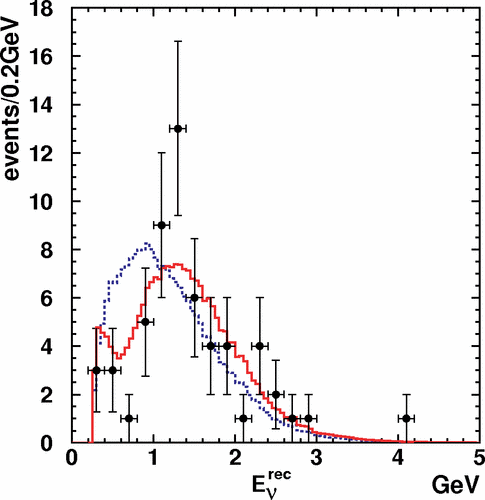
\includegraphics[width=0.45\textwidth]{intro_figures/k2k_oscillations.png}
  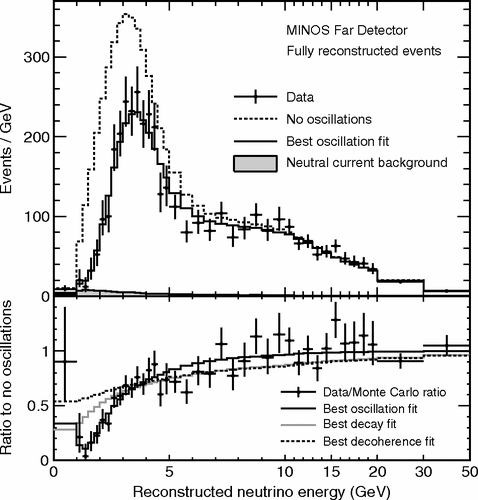
\includegraphics[width=0.45\textwidth]{intro_figures/minos_oscillations.png}
  \caption[MINOS and K2K \numu Oscillations]{(Left) K2K Event spectrum. (Right) MINOS event spectrum.  Both data sets clearly favor the oscillation hypothesis.}
  \label{fig:beam_oscillations}
\end{figure}

\subsubsection{Off-axis Neutrino Beams: T2K, \nova}
As one moves off of the axis of a neutrino beam, the flux from the beam decreases and narrows in energy.  For an oscillation experiment, a mono-energetic and point-like neutrino source is ideal, and an off-axis neutrino beam is closer to this ideal situation.  Both the T2K \cite{PhysRevLett.112.181801} and \nova \cite{PhysRevD.93.051104} experiments utilize this to study neutrino oscillations.  In particular, since \nova is fine grained detector, they are able to observe the appearance of electron neutrinos arising from \numu $\rightarrow$ \nue oscillations \cite{Adamson:2016tbq}.

\begin{figure}[htbp]
  \centering
  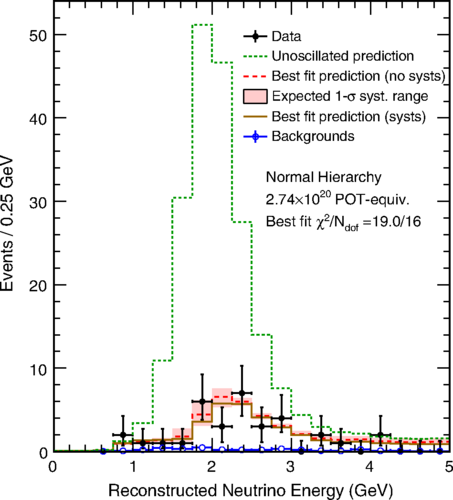
\includegraphics[height=2.5in]{intro_figures/nova_numu.png}
  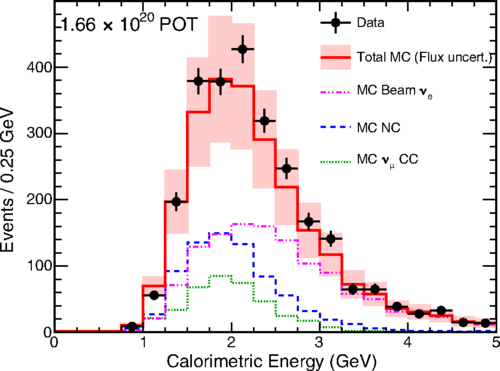
\includegraphics[height=2.5in]{intro_figures/nova_nue.png}
  \caption[\nova Oscillation Results]{(Left) \numu Oscillation results. (Right) \nue appearance oscillation results.  Figures from \cite{PhysRevD.93.051104} and \cite{Adamson:2016tbq}.}
  \label{fig:nova_oscillations}
\end{figure}

\subsubsection{Reactor Neutrinos and $\theta_{13}$}

The three neutrino oscillation paradigm requires three mass splittings (between the three neutrinos) and three mixing angles, however since it's observed that $\Delta m_{solar} = 7.6 \times 10^{-5}$, two of the mass splittings are effectively degenerate.  Measuring the mixing angles is slightly more complicated, however, in the regime where solar neutrino oscillations are not yet relevant the parameter $\theta_{13}$ can be measured effectively.  $\theta_{13}$ can be measured as non-zero from beam experiments such as MINOS, T2K and \nova \cite{PhysRevLett.107.181802, PhysRevLett.116.151806, PhysRevD.88.032002}, but it is directly measurable by searching for electron neutrino disappearance.  Nuclear reactors provide a high intensity flux of electron anti-neutrinos in the $\sim$ MeV range, so an experiment at around 1 km can probe \nuebar disappearance due to mass splittings in the range of $10^{-3} eV^2$.

The first experiment to actively search for \nuebar disappearance due to a nonzero $\theta_{13}$ mixing angle was CHOOZ \cite{Ardellier:2004ui} in France.  CHOOZ found no evidence for non-zero $\theta_{13}$, but set an upper limit on the mixing angle and proposed a follow up experiment to improve sensitivity to lower mixing angles \cite{Ardellier:2004ui}.

In 2012, a suite of experiments measured a non-zero $\theta_{13}$.  Double-CHOOZ \cite{PhysRevLett.108.131801}, Daya Bay \cite{PhysRevLett.108.171803}, and Reno \cite{PhysRevLett.108.191802} all report significant observation of \nuebar disappearance from reactor neutrinos, and Daya Bay and Reno results were at the $5\sigma$ level.  The latest results from Daya Bay \cite{An:2015rpe} show that the measurement of $\theta_{13}$ is at precision levels.  Though it is the last mixing angle measured, it is now the most well known.

\begin{figure}[htbp]
  \centering
  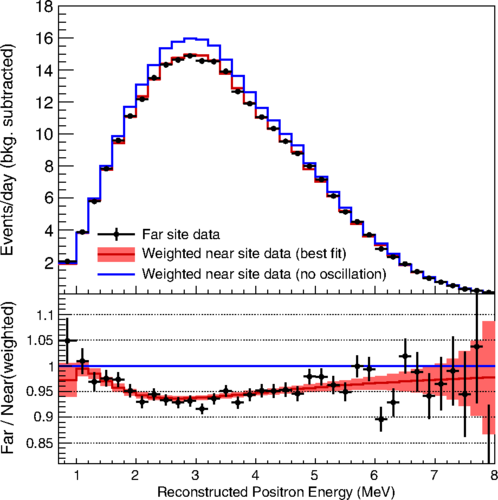
\includegraphics[width=0.45\textwidth]{intro_figures/daya_bay_spectrum.png}
  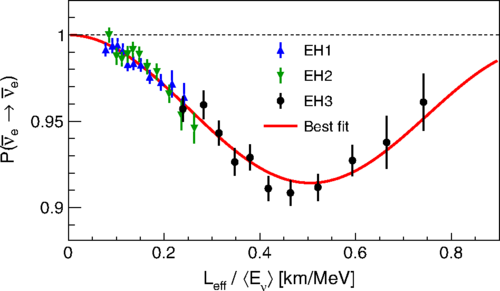
\includegraphics[width=0.45\textwidth]{intro_figures/daya_bay_survival.png}
  \caption[Daya Bay Oscillation Results]{(Left) Daya Bay prompt energy spectrum, showing a clear deficit. (Right) Daya Bay survival probability, showing the characteristic oscillation pattern of neutrino oscillations.}
  \label{fig:daya_bay_oscillations}
\end{figure}

\section{Future Directions in Neutrino Physics}
\label{sec:future_experiments}

Neutrino oscillations are a well established phenomenon.  Despite that, many properties of neutrinos remain elusive.  Some of intriguing puzzles that may be resolved experimentally soon are, for example, the direct measurements of neutrino mass \cite{BORNSCHEIN200514, Mertens:2014nha} by precision measurements of tritium decay.  Other experiments are probing whether or not neutrinos are their own anti-particle by searching for neutrino-less double beta decay \cite{Sisti:2015ayc, Auger:2012ar, 0954-3899-42-11-115201}.  Future experiments will be able to probe the mass heirarchy of neutrinos \cite{Abe:2011ts, Acciarri:2016ooe} as well as search for CP violation in the neutrino sector \cite{Acciarri:2016ooe, Ayres:2004js}.  Undoubtedly, the next decade will produce very exciting results in neutrino physics.

% DUNE and Nova for CP violation, experimental challenges, mass hierarchy, majorana or dirac, 



\chapter{Liquid Argon Time Projection Chambers}

\section{Time Projection Chambers}

The Time Projection Chamber, abbreviated TPC, is a revolutionary particle detector concept first proposed in 1974 by David Nygren at Lawrence Berkeley National Lab.  Since then, the TPC has found applications in a broad array of particle physics experiments such as collider experiments at the LHC \cite{Lippmann:2104844,Aamodt:2008zz}, precision measurements of muon properties \cite{Luo:2015oca}, dark matter experiments \cite{Akerib:2012ys,Aprile:2011dd} and more.  The abundance of uses for the TPC technology stems from the versatile and robust ability of a TPC to track charged particles.

In general, a Time Projection Chamber is a volume filled with some neutral and inert material.  Commonly, noble gases and liquids are used though this is not required.  An electric field is applied to the entire medium, and in some cases a magnetic field is applied as well.  The electric field is generally applied by using a high voltage cathode as one surface of the detector.  The opposing surface, the anode, is typically instrumented with readout equipment.

Time Projection Chambers are designed to observe electrically charged particles.  In particular, a high energy charged particle (such as an electron, muon, pion, proton, etc.) can travel through the detector medium and will ionize the substance as it passes through, leaving a trail of electrons and ions.  The applied electric field, emanating from the cathode, serves to separate the ionization electrons from the ions and move the electrons towards the anode of the detector.  The drifted electrons form the basis of the measurement of the particle.  In particular, they appear as a projection of the original track onto the anode of the detector, and the distance from the anode is determined by the time it took for the electrons to drift.  Hence the name, Time Projection Chamber.  Far more detail is given in the description of liquid argon TPCs, below \ref{sec:argoneut_detector}

\section{History and Liquid Argon Time Projection Chamber Concepts}

The Liquid Argon Time Projection Chamber (LArTPC) was initially proposed in 1977 by Carlo Rubbia \cite{Rubbia:1977zz}, who later led the development of the ICARUS detector and R\&D programs.  At the time of it's concept, neutrino physics was dominated by bubble chamber detectors like Gargamelle, renowned for it's remarkable resolution of particle topologies.  Initially, the LArTPC was proposed as a way to combine high spatial resolution detectors with calorimetry measuring detectors in a way that is scalable to massive detectors.  As the field of neutrino physics approaches the largest LArTPC to date with DUNE \cite{DUNE}, it's worthwhile to recall the original advantages of the LArTPC technology as laid out in 1977 \cite{Rubbia:1977zz}:

\begin{itemize}

\item{\bf ``It is dense''} : The relative high density of liquid argon, at 1.4 $g/cm^3$, provides a sufficiently high neutrino interaction rate such that high statistics measurements are feasible.

\item{\bf ``It does not attach electrons and permits long drift times''}: As a long drift time is essential to large scale detectors to both maximize the mass of the detector and minimize the number of readout channels, the fact that argon itself does not attach free electrons is an essential ingredient to LArTPCs.

\item{\bf ``It has a high electron mobility''}: The high mobility makes drifting electrons from particle ionization in a short time a feasible task.

\item{\bf ``It is cheap''}:  A detector can not be scaled to massive sizes unless the fundamental building block of the detector is affordable.

\item{\bf ``It is easy to obtain and purify''}: Purification challenges have largely been overcome for LArTPCs.  In particular, the \uboone experiment has demonstrated a viable way to achieve high purity argon without purging the detector of impurities first.

\item{\bf ``It is inert and can be liquified with liquid nitrogen''}: This makes the cryogenic systems for LArTPCs reasonable to purchase and implement.

\end{itemize}


40 years after the original proposal, it is remarkable how relevant the initial advantages remain in the face of an experiment such as DUNE. 

Since the original proposal, some additional advantages of LArTPCs have been noted and are worth mentioning.  For example, the scintillation of Liquid Argon has been successfully characterized and is measurable in coincidence with the drift ionization.  For large detectors, especially surface detectors, this allows the ability to match scintillation light to ionization tracks to reject out of time events such as cosmic particles.  It also allows the implementation of a hardware based trigger to filter neutrino interactions online.  For even modest sized LArTPCs, this can be an essential aspect to control data rates and ease computing requirements.

\section{Design of LArTPCs}
\label{sec:argoneut_detector}

As mentioned above, the Liquid Argon TPC has a long history of development.  This section presents the details of a modern LArTPC in it's design, given in the context of the \argoneut detector. A comprehensive and detailed description of the \argoneut detector is given in \cite{Anderson:2012vc}.

\subsection{\argoneut Time Projection Chamber}

The \argoneut TPC is a rectangular volume of liquid argon that measures 40 cm high (Y direction), 47 cm wide (X direction), and 90 cm long (Z direction).  In total, this corresponds to about 170 liters of Liquid Argon.  In it's running configuration, neutrinos from Fermilab's NuMI beam \ref{sec:numi_beam} enter nearly parallel to the Z direction, with a slight downward direction.  On the left side of the detector in the beam direction is the high voltage cathode providing a uniform electric field of 500 V/cm throughout the TPC (corresponding to approximately -23 kV of voltage at the cathode).  Opposite the cathode is the anode, composed of three wire planes, of which only two are instrumented for readout.

%insert argoneut tpc picture.
\begin{figure}[h]
  \centering
  \includegraphics[width=0.75\textwidth]{lartpc_figures/argoneut_tpc_and_cryostat.pdf}
  \caption{The \argoneut TPC positioned just outside of its cryostat.  The wire planes and the readout electronics are visible on the right side of the TPC.}
  \label{fig:argoneut_tpc}
\end{figure}

In the detector, as a neutrino interacts it produces outgoing particles, most commonly: muons, protons, neutrons, pions (charged and neutral), photons and electrons.  Naturally, the possible particles produced in a neutrino interaction is much broader than this short list, but this comprises the most frequent particles.  In the case of the electrically charged particles, the particle will ionize the argon atoms as it moves through the detector.  The ionization produced is a statistical quantity, but the average expected ionization depends strongly on the momentum and mass of the particle in question.  In general, particles with higher mass and lower momentum produce larger ionization per unit distance traveled \cite{bethe-bloch}.  The ionization per unit distance, measured most frequently in the units MeV/cm, is a very powerful tool for calorimetric identification of particles (as demonstrated in Chapter \ref{chp:electrons}.

Neutral particles, such as neutrons and photons, do not ionize the argon atoms as they traverse the detector.  However, these particles can still interact with the argon and produce charged particles visible to the TPC instrumentation.  Neutrons frequently will scatter off of an argon nucleus and produce a recoiling proton, which can be observed in the detector.  Photons can produce electromagnetic showers through Compton scattering and pair production, described more fully in Chapter \ref{chp:electons}.

After the particles from the neutrino interaction have produced ionization in the detector, the electric field separates the ions and electrons from each other.  Naturally, the separation is imperfect and depends on the strength of the electric field, the amount of ionization, as well as the angle of ionization with respect to the field.  This effect, known as recombination of electrons and ions, has been studied in detail in the \argoneut detector \cite{Acciarri:2013met}.  In general, this effect causes a quenching of the observed electrons compared to the true ionizing power of the high energy particles as seen in Figure \ref{fig:argoneut_recombination}.

The uniformity of the electric field in the \argoneut detector is maintained with a field shaping system of electrodes.  The electrodes are plated on  to the interior surface of the volume between the cathode and anode, and are held at a voltage linearly decreasing from cathode to anode.  In \argoneut, the field shaping strips are 1cm wide and seperated by 1cm, and there are 23 strips total.  This technique, however, is utilized in a variety of TPC experiments.

%insert dQ/dx vs dE/dx plot here.
\begin{figure}[h]
  \centering
  \includegraphics[width=0.5\textwidth]{lartpc_figures/recombination_dqdx_dedx.pdf}
  \caption{Measurement of the recombination effect in \argoneut using stopping protons, at 500 V/cm.}
  \label{fig:argoneut_recombination}
\end{figure}

Once the electrons have been separated from the ions, they drift towards the readout wires of the TPC.  Though argon itself does not attach electrons, impurities in the argon can do so.  The amount of drifting electrons declines as a function of the distance it has to drift.  This decline is well modeled with an exponential decline, and the decay constant is referred to as the electron ``lifetime.'' Proper calorimetry must take the lifetime of the electrons into account on hit by hit basis to correctly account for the effect of the impurities in the liquid argon.  In \argoneut, the electron lifetime is measured in data by comparing the amplitude of this at different drift distances as seen in Figure \ref{fig:argoneut_lifetime}.

%insert lifetime plot here.
\begin{figure}[h]
  \centering
  \includegraphics[width=0.5\textwidth]{lartpc_figures/argoneut_lifetime.pdf}
  \caption{The electron lifetime in \argoneut is computed run by run empirically, using a sample of depositions in the TPC from minimally ionizing particles.  Shown here is the fit, using an exponential, for run 648 giving an electron lifetime of 742 $\pm \mu s$ (statistical error only).}
  \label{fig:argoneut_lifetime}
\end{figure}


As alluded to above, the \argoneut detector has three planes of wires at the anode, two of which are instrumented.  The first plane, composed of 225 wires oriented vertically, serves as a shielding plane for the other wires and to provide shaping to the electric field through the TPC.  The three planes are spaced with 4mm between each other.  The second plane, referred to as the ``induction plane,'' contains wires that are set at +60$^o$ to the beam axis.  As electrons cross the shield plane, they approach the induction plane wires.  The wires are biased, however, such that the electrons drift around the individual wires.  The approaching and subsequent passing of electrons induces a current on these wires (hence the name ``induction plane'') and bipolar pulse shape is recorded by the readout electronics for wires that observe electrons.  See figure \ref{fig:argoneut_signals} for examples of this pulse.

The final set of wires, dubbed the ``collection plane,'' is biased such that it collects the drifting electrons onto it and they are observed as a pulse of charge by the electronics system.  The collection plane is set at an angle of -60$^o$ to the beam direction.  The two instrumented planes each have wire spacings of 4mm, and sample at 5.05 MHz.  In total, the instrumented planes have 240 wires in each plane.  Naturally, since the wires are at an angle with respect to the TPC axes, not all wires are of the same length.  Most wires, 144 of 240 in each plane, are 46.2 cm long.  The shortest wires are 3.7 cm long.

The sense wires are readout with a system of electronics sampled every 198 ns, and the readout system has a sensitivty of 7.49 ADC/fC of charge recorded.  This gives a signal to noise ratio of 15 or higher for minimally ionizing particles in the TPC.  An in depth description of the \argoneut readout electronics is available in \cite{Anderson:2012vc.}


%insert wire pulse figure
\begin{figure}[h]
  \centering
  \includegraphics[width=\textwidth]{lartpc_figures/argoneut_signal.pdf}
  \caption{Raw and deconvoluted signal shapes from the \argoneut detector.  On the top is shown the induction pulse.  The bipolar shape of the pulse in the induction plane is corrected during the deconvolution stage.  On both planes, a Gaussian hit fitting technique is used to determine the amount of charge recorded. Figure from \cite{Anderson:2012vc}.}
  \label{fig:argoneut_signals}
\end{figure}

\section{Event Imaging and Reconstruction}

Each wire measures a signal of electrons as they drift, as a function of time.  When the wires are arrayed in an image in sequential order, such that the x axis is wire number and the y axis is time tick, 2D images are formed such as in figure \ref{fig:argoneut_data}.  As seen in figure \ref{fig:argoneut_projection}, the wire planes represent projections of the 3D data onto a plane that is orthogonal to the wires themselves.

%insert argoneut data picture.

%insert argoneut projection picture
\begin{figure}[h]
  \centering
  \includegraphics[width=\textwidth]{lartpc_figures/argoneut_plane_projection.pdf}
  \caption{Representation of the projection of the LArTPC in \argoneut.  The wire and time axes give a 2D image that represents a projection of the 3D charge depositions on to the 2D surfaces shown in blue.  Figure from \cite{Anderson:2012vc}.}
  \label{fig:argoneut_projection}
\end{figure}

\subsection{Deconvolution}
The reconstruction of these images into a 3D event starts at the lowest level, filtering and deconvolution of the wire signals.  In general, the number of electrons recorded by a given wire as a function of time is not prefectly matched by the ADC signals read out by the detector.

To correct for this, a deconvolution process is applied to each wire.  As seen in figure \ref{fig:argoneut_signal_shaping}, the response of the detector to a delta function introduces a spread of signal which is removed using a scheme with the Fast Fourier Transform. The response of each channel is measured with external pulse generators.  The convolution theorem then allows the removal of the detector response by taking the  inverse Fourier transform of $\frac{v[t]}{r[t]}$, where $v[t]$ is the Fourier transform of the recorded waveform and $r[t]$ is the Fourier transform of the channel's response.  Figure \ref{fig:argoneut_deconvolution} shows the result of applying deconvolution to \argoneut data in the collection and induction planes.  In addition, the deconvolution for the induction plane removes the bipolar behavior to make hit finding easier.

% need an image of argoneut deconvolution

\begin{figure}[h]
  \centering
  \includegraphics[width=\textwidth]{lartpc_figures/argoneut_signal_shaping.pdf}
  \caption{On the left, an image of the idealized detector response to drift electrons in the induction and collection plane.  On the right, the response of the electrons filter and digitization to a delta function pulse.  Figure from \cite{Anderson:2012vc}.}
  \label{fig:signal_shaping}
\end{figure}

\subsection{Hit Finding}

For each wire in the detector, a hit finding algorithm is used to locate the regions of the readout with electron deposition signals.  While there are several different hit finding algorithms available in LArSoft \cite{larsoft}, the official LArTPC reconstruction software, the all follow a generalized procedure.

First, a deconvolved (and noise filtered) wire signal is scanned for regions of signal above a specified threshold.  Often, the baseline threshold of hit finding depends on whether the signal is from collection or induction planes.

Next, the regions of interest are fitted with an analytic function to allow a precise determination of the time tick, peak, and integral of the charge deposited.  The most common function used is a Gaussian.  In some cases, and commonly in neutrino interactions, hits that are close to each other from different particles will have overlapping regions.  In this case, the multiplicity of the region above threshold can be determined to help tracking algorithms accurately distribute hits between different particles.  An example of this is seen in Figure \ref{fig:argoneut_hit_multiplicity}.  In general, complicated regions with multiple hits are fit with several Gaussians summed together.

\begin{figure}[h]
  \centering
  \includegraphics[width=\textwidth]{lartpc_figures/argoneut_hit_multiplicity.pdf}
  \caption{A neutrino vertex as seen in the induction view in \argoneut.  The top left shows the reconstructed signals above threshold.  The other figures show the wire signal moving away from the vertex: the initial signal is wider than normal, and as the tracks diverge in the detector the two peaks are resolved.  Figure from \cite{Anderson:2012vc}.}
  \label{fig:argoneut_hit_multiplicity}
\end{figure}

\subsection{Cluster, Tracking and 3D Reconstruction}

Once the wire signals have been deconvolved, and the signal depositions have been reconstructed as hits, a number of higher level steps remain between hits and physics data.  First, hits must be grouped together based on which particle they originated from.  In general, this is an extremely difficult problem with no simple answer.  For particles like muons and protons, which produce simple tracks of hits in the detector, it is not impossible and a lot of progress and achievements have been made.  For more complicated events, such as electromagnetic showers, clustering remains the weakest point of the reconstruction chain.

For a track like particle, in general, the groups of hits are associated together into clusters.  These cluster are then matched across the planes of the detector (two planes in argoneut, but many state of the art detectors have 3).  Though the planes offer different projections of the 3D events into 2D, the drift direction (time tick direction in \ref{fig:argoneut_data}) is a common axis in every projection.  Therefore, the most useful metric to determine if two clusters are from the same track in the argon is the time if took those clusters to drift to the wires.

Once clusters from multiple planes have been matched together, the wire information between the two clusters can be used to determine where in the Y-Z plane the clusters overlap.  This is because each wire intersects the other plane's wires at most once, so if a charge deposition from one plane is matched to one on another plane, it uniquely determines the location of the 3D charge (The X coordinate comes from the drift time).

Almost all of the details of 3D tracking and reconstruction have been skimmed here, as they are not crucial to the work presented in this thesis.  However, a great detail of knowledge and techniques is reported in many references \cite{reco:tracking_ref} \cite{reco:other_refs.}

\subsection{Particle Identification and Calorimetry}

In a LArTPC, the calorimetric identification of particles is based upon the behavior of charged particles moving through the argon.  The energy deposited per centimeter is dictated by the Bethe-Bloch equations, and the properties in argon of common particles are seen in Figure \ref{fig:bethe_bloch}.

As a particle loses energy, it's amount of ionization decreases until it reaches a minimum before the ionization spikes to very high values.  Due to the limited resolution of the detector, however, the observed dE/dx values for a given particle will increase as the particle comes to a rest.  As seen in Figure \ref{fig:residual_range}, this measure of dE/dx versus residual range allows calorimetric separation of particles.  In particular, protons are easily separated from muons and pions with this measure.

\begin{figure}[tb]
  \centering
  \includegraphics[]{lartpc_figures/residual_range.pdf}
  \caption{Caption here}
  \label{fig:residual_range}
\end{figure}

Since LArTPCs also offer bubble chamber quality images, the topology of an event can give excellent ways to distinguish particles.  As seen in Figure \ref{fig:mu_pi}, particles like muons and pions that are difficult to distinguish with calorimetry can often be separated based on subsequent interactions within the TPC.



\section{MINOS}

\argoneut is fortunate in that it is located directly upstream of the MINOS near detector, which is a magnetized tracking detector \cite{MINOS}.  This gives \argoneut a distinct trait that no other LArTPC has had: muon sign selection for muons produced in \argoneut that enter the MINOS near detector.


\begin{figure}[h]
  \centering
  \includegraphics[width=\textwidth]{lartpc_figures/minos.pdf}
  \caption{An event display depicting the \argoneut experiment and the MINOS near detector. \argoneut is the small box in the foreground.  The tracks represent TPC data of \numu CC interactions that were successfully tracked and matched into the MINOS near detector.  Figure from \cite{Anderson:2012vc}.}
  \label{fig:signal_shaping}
\end{figure}

\argoneut is only 90cm long at it's longest dimension, and since the NuMI beam has neutrino energies of 10+ GeV, it is extremely rare for muons produced in \argoneut to stop within the detector.  This enabled several precision measurements of muon neutrino cross sections on argon by looking for neutrinos that interact in \argoneut, and tracking them through the MINOS near detector \cite{argoneut_numu}, \cite{argoneut_antinumu}.

For the analyses presented in this thesis, MINOS is not used as a muon spectrometer directly.  Instead, since the target interaction is electron neutrinos, MINOS is able to provide rejection of muon neutrino events.


\chapter{\label{chp:beams} Neutrino Beams}

Direct measurements of neutrinos have two parts: a source of neutrinos, and a detector to observe them.  The most precise experiments required detailed knowledge of the workings of both the source {\em and} the detector.  This chapter describes the important components of the Fermilab accelerator based neutrino beams.  The Booster Neutrino Beam (BNB) is relevant to the Fermilab Short Baseline Neutrino Program, in Chapters~\ref{chp:sbn} and \ref{chp:systematics}.  The Neutrinos from the Main Injector (NuMI) beam is relevant for the \argoneut experiment in Chapter~\ref{chp:emshowers}. 

\section{Accelerator Based Neutrinos}

A popular source of neutrinos in modern experiments are the neutrinos from accelerator complexes.  As of the writing of this thesis, there are three active neutrino beams: two at Fermilab \cite{Adamson:2015dkw, AguilarArevalo:2008yp}, and one in Japan \cite{Abe:2014oxa}.  Compared to other sources of neutrinos, accelerator based neutrinos offer some advantages.

First, neutrino beams made at accelerator complexes are designed, and not a by-product of other circumstances.  This means that the design of the beam is often optimized for physics goals, in particular by tuning the energy spectrum and energy range of the neutrino beams.  Combined with intelligent positioning of detectors, accelerator neutrino beams can be optimized to probe a vast range of oscillation signals.

The NuMI beam, described below, was designed to have three modes of running to cover an entire energy range from 1 to 20 GeV neutrinos.  In general, accelerator based neutrino sources are crafted to build neutrino beams that will allow the neutrino experiments in the beam to maximize their physics output.

Another advantage to neutrino beams at accelerators is the pulse structure of the beam.  Since accelerators, like Fermilab, make neutrino beams by colliding bunches of protons with a target material, the timing of the proton bunches provides a natural time structure to the neutrino beams.  Downstream detectors can, using sufficiently time-sensitive detection material, ``time-in'' to the neutrino beam pulses to reject non beam backgrounds.  For experiments on or near the surface, this is exceptionally important for rejecting cosmic backgrounds.

\section{Fermilab's Accelerator Complex}

At Fermilab, where two of the three active neutrino beams originate, much of the physics program is derived from the use of the proton beam that Fermilab produces.  All of the proton beams, regardless of destination, start in the same location.  A bottle of hydrogen provides a source of protons for the entire accelerator complex.  In batches, some of the hydrogen atoms are given a negative charge by the addition of an electron, and these electrons are pushed into the Linear Accelerator (LINAC) at Fermilab with 750 KeV of energy (via a Cockroft-Walton generator).  The LINAC accelerates the protons to 400 MeV, and at the end of the LINAC the protons enter the Booster, a synchrotron.  Before entering the Booster, the electrons are knocked off of the H$^-$ ion to ensure that only protons enter the downstream accelerator system.  Over the course of thousands of rotations around the Booster, the protons are accelerated to 8 MeV of kinetic energy.

The Booster can nominally operate at 15 Hz, though is generally run at lower frequencies.  Future upgrades to Fermilab's accelerator complex involve running the Booster at it's maximum rate to produce as many protons as possible.  From the Booster, protons can be extracted to the Booster Neutrino Beam target, described below (Section~\ref{sec:bnb}).  The majority of protons, however, enter the Main Injector to be accelerated to higher energies.  The Main Injector can accelerate protons to 120 GeV.

At the time of writing, the majority of the protons from the main injector are used in the NuMI beam (Section~\ref{sec:numi_beam}), while some are used for fixed target experiments and test beams (beams made of pions or other particles, generally secondary or tertiary beams from the proton beam).  At the time of the data collected for this analysis, however, some of the protons from the Main Injector were used to produce anti-protons for the Tevatron, and some were injected into the Tevatron directly.  In the future, it's excepted that a large fraction of protons will be used for the muon campus (for mu2e and g-2 \cite{Bartoszek:2014mya} \cite{Grange:2015fou}), and further protons will be used for the LBNF Neutrino Beam \cite{DUNE}.

\section{Booster Neutrino Beam}
\label{sec:bnb}

The Booster Neutrino Beam (BNB) is Fermilab's lower energy neutrino beam, and the primary beam of \MB, \uboone, and the Short Baseline Neutrino Program (see Chapter \ref{chp:sbn}).  The BNB is one of the most well understood, extensively studied neutrino beams in existence, and has been running since the \MB experiment and is expected to run until past 2020.

\subsection{Booster Neutrino Beam History}
The BNB was designed for, and by, the \MB collaboration.  \MB was a Cherenkov style detector, searching for electron neutrino appearance.  Because the primary background for \MB was photons from neutral pion production in the detector, which come from higher energy neutrinos, the BNB flux was designed to suppress neutrinos with energy above $\approx$ 1 GeV.

The origin of the BNB is 8 GeV protons (8.89 GeV/c momentum) from Fermilab's Booster complex.  These protons are transported to a Beryllium target, encased in a magnetic focusing horn.  The protons collide with the Be and produce hadrons within the target, which are focused into the forward direction by the focusing horn.  The hadrons enter a decay pipe of 50 meters, where they decay in flight into lighter particles including neutrinos.  At the end of the decay pipe is a beam stop to prevent all particles (except neutrinos) from proceeding.  A schematic of the proton entry, horn location, decay pipe and beam stop are shown in Figure~\ref{fig:mb_target_schematic}.

\begin{figure}[tb]
  \centering
  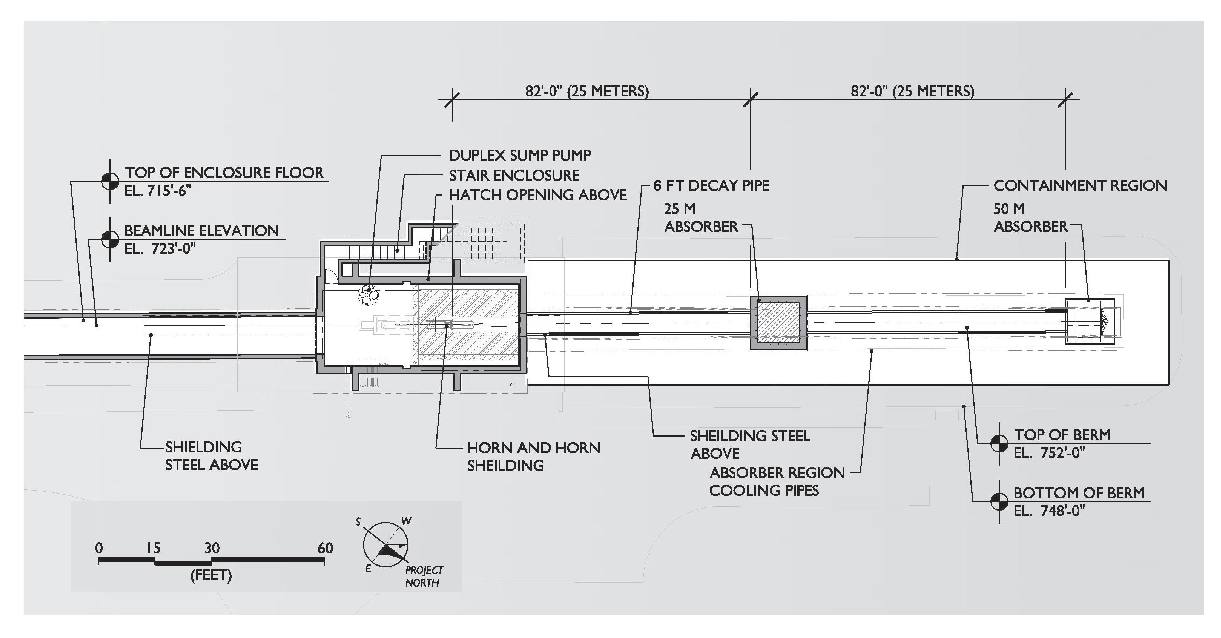
\includegraphics[width=\textwidth]{beams_figures/mb_target_schematic}
  \caption[BNB Target Schematic]{The Booster Beam target hall and decay pipe.  Protons enter from the left, and hadrons decay in the decay pipe for up to 50m before the beam stop.  \MB, \uboone, and the other SBN experiments are to the right. Figure from \cite{AguilarArevalo:2008yp}}
  \label{fig:mb_target_schematic}
\end{figure}

The batches of protons delivered to the Booster target are pulsed, typically at a rate not more than 5 Hz, and each bunch is approximately 1.6$\mu$s in duration.  For downstream experiments, such as \MB and the SBN Program, the ability to resolve interactions in the detector on the time scale of 1.6 $\mu$s is extremely useful for rejecting out-of-beam-time cosmics.  

Each bunch of protons from the Booster typically contains approximately 4e12 protons.  These protons collide with the Beryllium target, which is 71 centimeters long and made from seven segments of Beryllium.  This length corresponds to 1.7 interaction lengths for the protons, meaning that just over 80\% of the protons interact in the target material.  The number of protons on target is measured upstream of the target by two magnetic toroids, and the uncertainty on the number of protons delivered is on the order of 1-3\% typically.

Upon interacting, the protons produce lighter hadrons such as pions and kaons.  The spectra of produced hadrons is the source of the largest uncertainty in the Booster Neutrino Beam, and is discussed in more detail in Section~\ref{section:flux_uncert}.  The hadrons produced by the protons at the target are focused with the magnetic horn which produces an azimuthal, pulsed magnetic field in time with the proton delivery.  The primary source of the neutrinos in the BNB is from decay in flight pions, though there is significant contamination from kaon decay and muon decay (where the muons are also the product of pion decay).  The kaons and muons also produce a contamination of electron neutrinos in the primarily muon neutrino beam, and this flux of electron neutrinos is the primary background in the Short Baseline Neutrino Program's \nue appearance analysis (see Section~\ref{subsection:event_reco}.

The estimation of the flux, by neutrino type and by originating particle, at the \MB location can be seen in Figure~\ref{fig:mb_flux_nu}.  This estimate of the flux is produced with a sophisticated Monte Carlo simulation, discussed in detail in \cite{AguilarArevalo:2008yp}.  However, the general procedure is:

\begin{enumerate}

\item{Define the beamline geometry, including the shape, location, and composition of the components of the BNB.  This includes the target, magnetic horn, decay pipe and beam stop as well as the other minor parts.  The simulation attempts to capture the reality of the beam construction as closely as possible.  A graphical representation of the magnetic focusing horn can be seen in Figure~\ref{fig:mbhorn}.}

\item{Generate protons in the simulation that match the expected protons from the beam, accounting for the optical effects of the beam upstream of the target.}

\item{Simulate the interaction of protons in the target and surrounding material.  Substantial effort was made by the \MB collaboration to constrain this step of the simulation, as it is the primary source of systematic uncertainties in the beam model.  Dedicated experiments, such as HARP \cite{Catanesi:2007ab} and BNL E910 \cite{Chemakin:2007aa}, are used to constrain pion production and improve the flux prediction, as the uncertainties in pion production dominate the flux uncertainties.}

\item{Propagate particles from the primary interactions using GEANT\cite{Agostinelli:2002hh} to account for energy loss and interactions that change the kinematics of the particles above.  This also includes accounting for the focusing effects of the magnetic horn.}

\item{Identify particles that result in neutrinos at the detector, accounting for branching ratios and kinematic distributions properly.  Statistical boosting techniques are also used, since the solid angle subtended by the neutrino detector is small in the lab frame of the decaying particles.}

\end{enumerate}

\begin{figure}[tb]
  \centering
  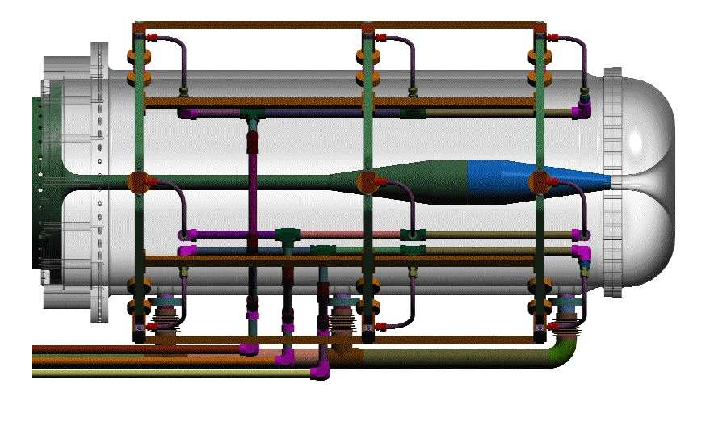
\includegraphics[width=\textwidth]{beams_figures/mbhorn}
  \caption[BNB Horn and Focusing Magnet]{The Booster Beam horn and focusing magnet.  Figure from \cite{AguilarArevalo:2008yp}}
  \label{fig:mbhorn}
\end{figure}

\begin{figure}[tb]
  \centering

    \begin{subfigure}[t]{0.5\textwidth}
        \centering
        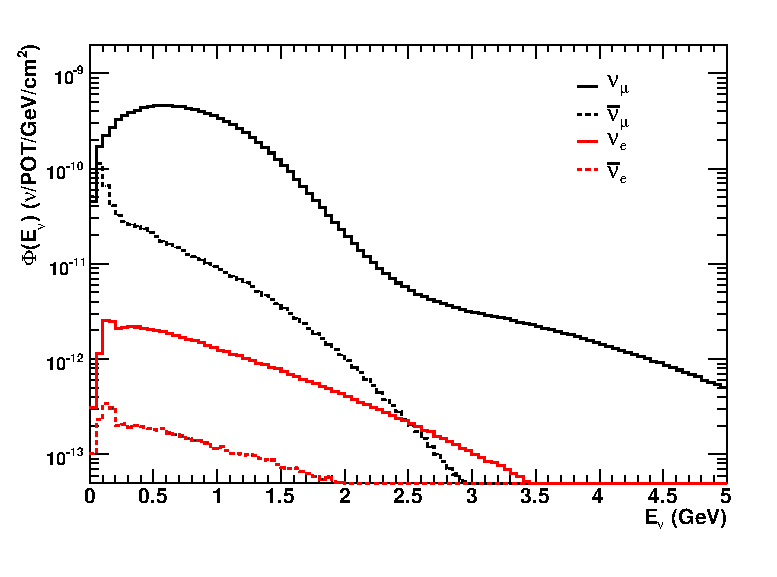
\includegraphics[height=2in]{beams_figures/mb_flux_nu}
    \end{subfigure}%
    ~ 
    \begin{subfigure}[t]{0.5\textwidth}
        \centering
        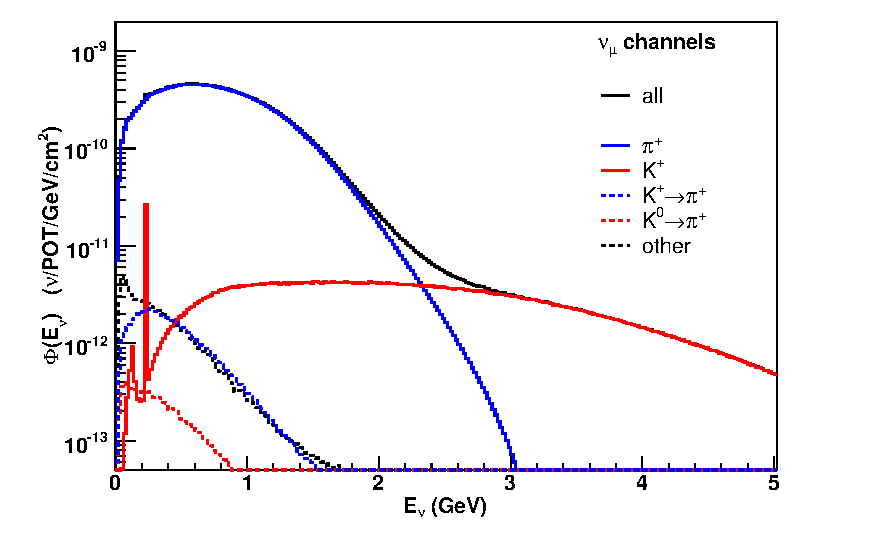
\includegraphics[height=2in]{beams_figures/mb_flux_by_type_nu}
    \end{subfigure}
  \caption[\MB Flux]{(Left) Total predicted flux at the MiniBooNE detector by neutrino species with horn in neutrino mode. (Right) Muon neutrino flux by type of original particle. Figure from  \cite{AguilarArevalo:2008yp}}
  \label{fig:mb_flux_nu}
\end{figure}

The work covered in this document does not use the \MB detector at all, however it does leverage the \MB flux calculation machinery to simulate the flux at multiple locations for the Short Baseline Neutrino Program, shown in Figure~\ref{fig:sbn_flux}.  In this light, the discussion of the systematic uncertainties of the flux prediction are left to Section~\ref{section:flux_uncert}.  However, Table~\ref{tab:mb_flux_uncert} is included here to showcase the precision at which \MB constrained the BNB, an accomplishment that future experiments are building upon.

\begin{figure}[htbp]
  \centering
  \includegraphics[width=0.45\textwidth]{beams_figures/bnb_flux_nu_100m.eps}
  \includegraphics[width=0.45\textwidth]{beams_figures/bnb_flux_nu_470m.eps}
  \includegraphics[width=0.45\textwidth]{beams_figures/bnb_flux_nu_700m.eps}
  \caption[BNB Fluxes]{The neutrino flux from the Booster Beam at the three locations of the SBN Program.  The flux falls at approximately $1/r^2$, however, the near detector flux is slightly distorted due to its proximity to the decay pipe.}
  \label{fig:sbn_flux}
\end{figure}

\begin{table}[tb]
  \caption{Fractional flux uncertainties, by species of neutrino, from the \MB flux calculation.}
  \centering

  \begin{tabular}{l|rrrr}
  \hline
  \hline
  Source Of Uncertainty & \textbf{\numu} & \textbf{\numubar} & \textbf{\nue} & \textbf{\nuebar}  \\
  \hline
     Proton Delivery        &  2.0\% &  2.0\% &  2.0\% &  2.0\% \\
     Proton Optics          &  1.0\% &  1.0\% &  1.0\% &  1.0\% \\
     $\pi^+$ Production     & 14.7\% &  1.0\% &  9.3\% &  0.9\%\\
     $\pi^-$ Production     &  0.0\% & 16.5\% &  0.0\% &  3.5\% \\
     $K^+$ Production       &  0.9\% &  0.2\% & 11.5\% &  0.3\% \\
     $K^-$ Production       &  0.0\% &  0.2\% &  2.1\% & 17.6\% \\
     Horn Field             &  2.2\% &  3.3\% &  0.6\% &  0.8\% \\
     Nucleon Cross Sections &  2.8\% &  5.7\% &  3.3\% &  5.6\% \\
     Pion Cross Sections    &  1.2\% &  1.2\% &  0.8\% &  0.7\% \\
  \hline

  \hline
  \end{tabular}
  \label{tab:mb_flux_uncert}
\end{table}


\section{Neutrinos from the Main Injector (NuMI Beam)}
\label{sec:numi_beam}

The Neutrinos from the Main Injector (NuMI) beam was conceived of with the MINOS (Main Injector Neutrino Oscillation Search) experiment at a time when neutrino oscillation parameters were not well constrained.  In particular, there were hints that the atmospheric mass splitting was of the order of magnitude of $10^{-3} eV^2$, but more than that was unknown.  Therefore, the NuMI beam was designed to be configurable and to run in multiple modes of running: Low Energy, Medium Energy, and High Energy.  The various energy spectra are shown in Figure~\ref{fig:numi_spectra}.  A comprehensive discussion of the design and operation of the NuMI beam is available in Ref. \cite{Adamson:2015dkw}.  This section will be a very brief summary of some important facts about the NuMI beam.

\begin{figure}[htbp]
  \centering
  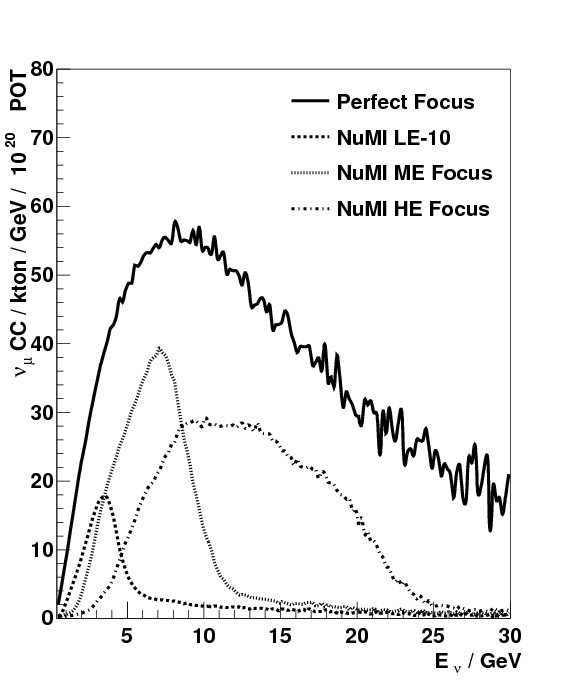
\includegraphics[width=0.45\textwidth]{beams_figures/numi_focus_vs_perfect.png}
  \caption[NuMI Energy Modes]{The various energy tunings for NuMI.  The analysis performed for this work is based off of the Low-Energy mode, mainly in anti-neutrino mode.}
  \label{fig:numi_spectra}
\end{figure}

The NuMI target is similiar to the BNB target, above, though it is more complex for several reasons.  First, the distance between the target itself and the focusing horns is adjustable to allow the different running configurations.  Additionally, there are two focusing horns instead of just one.  The first horn, located close to the target, and the second horn, downstream, effectively act as a charged hadron focusing system.  With a higher energy source of protons compared to the BNB, the two horns are necessary to focus the higher energy secondary particles from the target.  Downstream of the target and horn area is the NuMI decay pipe, which is 675m in length.  After the decay pipe there is 240m of rock, followed by the near detector for MINOS.  \argoneut, the detector that collected the data of this thesis, is located in the MINOS near detector hall in between MINOS and Miner{$\nu$}a.
The schematic of the target, horn, and decay pipe are shown in Figures~\ref{fig:numi_horn}.

\begin{figure}[htbp]
  \centering
  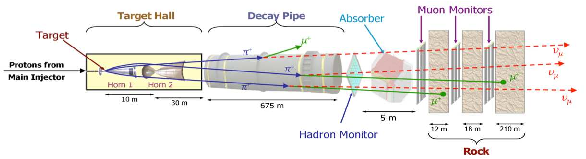
\includegraphics[width=0.95\textwidth]{beams_figures/numi_beam_target.png}
  \caption[NuMI Beam Target]{The beam target, horns, and decay pipe are shown for NuMI.}
  \label{fig:numi_horn}
\end{figure}

The NuMI flux is simulated with a FLUKA simulation in a way very similar to the BNB.  It also benefits from the constraints from dedicated hadron production experiments \cite{Nigmanov:2009zz, Alt:2006fr}, and in situ measurements from the detectors along the beam line \cite{Aliaga:2016oaz}.  The flux models in the simulation of the beam are generally accurate to with 10 or 20\%, however experimental constraints and flux tunings can decrease the uncertainty to less than 10\% \cite{Aliaga:2016oaz}.  The flux shown in Figure~\ref{fig:argoneut_flux} is the computed \argoneut flux without the addition of the constraints, in the NuMI Low Energy mode.  Since the result presented in this thesis is not a cross section measurement but a detection of electron neutrinos, the tuned  flux is unnecessary precision for this result.

\begin{figure}[htbp]
  \centering
  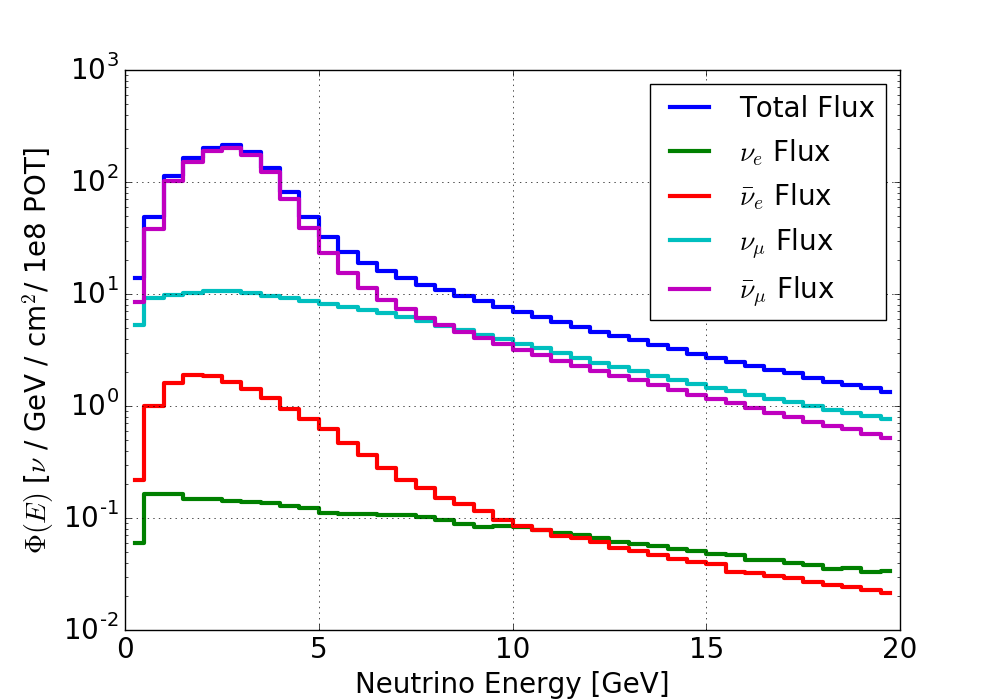
\includegraphics[width=0.45\textwidth]{beams_figures/argoneutFlux.png}
  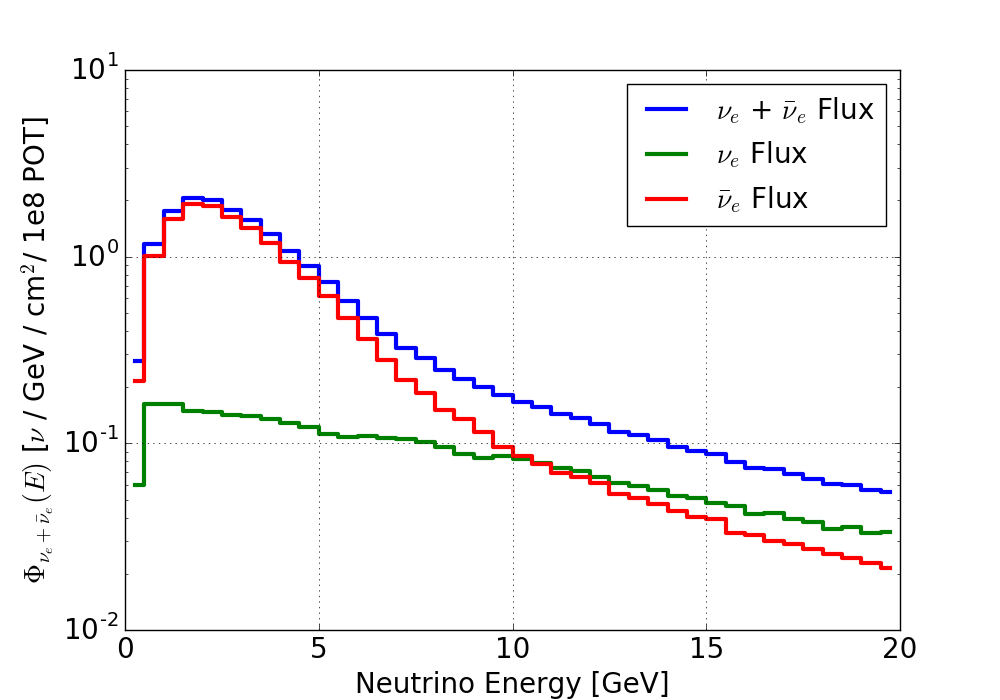
\includegraphics[width=0.45\textwidth]{beams_figures/argoneutFlux_nue.png}
  \caption[NuMI Flux at \argoneut]{The predicted flux at \argoneut.  (Left) All flavors of neutrino species. (Right) Only the electron neutrino and anti-neutrino flux.}
  \label{fig:argoneut_flux}
\end{figure}




\chapter{Short Baseline Neutrino Program}
\label{chp:sbn}

This chapter will describe the Short Baseline Neutrino Program, and the anomalies it is seeking to resolve.

\section{Motivation and Goals}

Over the past two decades, experimental hints of beyond the Standard Model neutrino physics have appeared in several distinct subfields of neutrino experiments.  Taken together, the constitute hints at oscillation physics on mass splitting scale that is inconsistent with the known oscillations models.  This section will briefly summarize the current anomalies in this area of neutrino oscillations, known as Short Baseline oscillation physics.

A more thorough analysis of the global, experimental picture of neutrino oscillations is given by oscillation analyses such as Kopp et. al \cite{Kopp:2013vaa}, Giunti et. al \cite{Giunti:2013aea}.  Though there is tension in the experimental evidence, there is indication that anomalous neutrino oscillation is occurring at short baselines.


\subsection{LSND}

In 1995, the Liquid Scintillator Neutrino Detector at Los Alamos National Laboratory published the results of it's first search for \numubar to \nuebar oscillations \cite{Athanassopoulos:1995iw}.  The detector was a liquid scintillator detector making observations of electron anti neutrinos through the inverse beta decay reaction on carbon.  The origin of the neutrinos was a decay at rest pion source, producing neutrinos in the range of 20 to 50 MeV.  In the inverse beta decay reaction signature is a prompt positron emission, followed by a 2.2 MeV gamma from neutron capture.   LSND observed 89.7 $\pm$ 22.4 $\pm$ 6.0 \nuebar candidate events above background over five years of data taking, corresponding to a significance of 3.8 $\sigma$.


\begin{figure}[htbp]
    \centering
    \begin{subfigure}[t]{0.5\textwidth}
        \centering
        \includegraphics[height=3in]{sbn_figures/lsnd_beam_excess}
    \end{subfigure}%
    ~ 
    \begin{subfigure}[t]{0.5\textwidth}
        \centering
        \includegraphics[height=3in]{sbn_figures/lsnd_allowed_region_by_lsnd.pdf}
    \end{subfigure}
    \caption[LSND Excess]{ (Left) Excess of candidate \nuebar events observed by LSND, plotted as a function of L/E of the reconstructed neutrino. (Right) Allowed region of oscillation parameters when fit against a 2 neutrino mixing model.}
   \label{fig:lsnd_beam_excess}
\end{figure}

As seen in Figure~\ref{fig:lsnd_beam_excess}, the LSND excess is inconsistent with the three neutrino oscillation paradigm.  Instead, it hints at oscillations at L/E of $\sim$ 0.5 and a mass splitting of $\sim$ 1 eV$^2$.  For comparison, the  solar and atmospheric mass splittings are in the ranges of $7\times10^{-5}\text{ eV~}^2$ and $2\times10^{-2}\text{ eV~}^2$, respectively.

\subsection{Reactor Experiments}

Many experiments have measured the flux of neutrinos from nuclear reactors over many years.  However, a recent reevaluation \cite{Huber:2011wv} \cite{Mueller:2011nm} of the expected neutrino flux from reactors has led to an observed deficit in historical measurements, as seen in Figure~\ref{fig:reactor_deficit} \cite{Mention:2011rk}.  This deficit, at the level of 6 to 7\%, is consistent with an oscillation of reaction \nuebar into an unobserved sterile state.

Some concern over the so called Reactor Deficit has been raised over the fact that before the recalculation was completed, all experiments were in agreement with the existing theoretical prediction.  However, experimental results from the Daya Bay collaboration \cite{An:2015nua}, done in a blind analysis, support the experimental evidence of the reactor neutrino deficit (See Figure~\ref{fig:daya_bay_reactor_flux}).

\begin{figure}[htbp]
  \centering
  \includegraphics[width=\textwidth]{sbn_figures/reactor_flux.pdf}
  \caption[Reactor Deficit]{Measurements of the reactor neutrino flux indicate a deficit when compared with theoretical predictions.  It's plausible that the deficit is evidence of anomalous neutrino oscillations.}
  \label{fig:reactor_deficit}
\end{figure}

\begin{figure}[htbp]
  \centering
  \includegraphics[]{sbn_figures/daya_bay_flux_deficit.pdf}
  \caption[Daya Bay Reactor Flux]{The Daya Bay experiment performed a blind measurement of the reactor flux and their location and found excellent agreement with previous experimental data.  This was performed after the flux recalculations.}
  \label{fig:daya_bay_reactor_flux}
\end{figure}

% \subsection{Source Experiments}

% For measurement of Solar Neutrinos, the experiments GALLEX and SAGE both used radioactive sources as a neutrino source for calibration.

% \cite{Abdurashitov:1998ne} \cite{Hampel:1997fc}

\subsection{\label{sec:miniboone} \MB}

Most recently, the \MB collaboration published evidence for an excess of electron neutrino candidate events in both neutrino and anti neutrino mode at Fermilab's Booster Neutrino Beam \cite{Aguilar-Arevalo:2013pmq}.  Their results, shown in Figure~\ref{fig:mb_stacked_rates}, clearly indicate an excess of candidate events.  Despite the significance of the results (3.4 $\sigma$ for Neutrino Mode, 2.8 $\sigma$ in Anti-Neutrino Mode), the \MB results are particularly controversial.

First, the detector technology of \MB is a Cherenkov type detector, meaning that it distinguishes particles based upon their Cherenkov signature observed by PMTs at the outer surface of the detector.  Since electrons and photons both produce similar electromagnetic cascades, \MB is unable to distinguish between electron and photon events.  For the electron neutrino analysis in Figure~\ref{fig:mb_stacked_rates}, this implies that the excess can not be attributed as electron neutrinos without further investigation, and therefore isn't conclusively inconsistent with the standard three neutrino oscillation model.  It's worth mentioning, however, that the excess is significant enough to warrant \uboone's investigation, discussed in detail below.

Second, the \MB oscillation result is inconsistent with anticipated 3+1 model sterile neutrino oscillation signals.  As seen in Figure~\ref{fig:mb_stacked_rates}, the observed excess can not simultaneously be interpreted as electron neutrinos from muon neutrino oscillations (through a sterile state) while agreeing with the sterile neutrino oscillation model.

Despite the controversy, when taken with consideration into consideration with other results such as LSND (at the same L/E as \MB), and the reactor and source anomalies, there is intriguing evidence of physics beyond the Standard Model in the neutrino sector.


\begin{figure}[htbp]
  \centering
  \includegraphics[]{sbn_figures/miniboone_beam_excess.pdf}
  \caption[\MB Beam Excess]{Caption here}
  \label{fig:mb_beam_excess}
\end{figure}

\begin{figure}[htbp]
  \centering
  \includegraphics[]{sbn_figures/miniboone_stacked_rates.pdf}
  \caption[\MB Stacked Rates]{Caption here}
  \label{fig:mb_stacked_rates}
\end{figure}

\subsection{Global Fits}
\label{sec:global_fits}

With many hints at beyond the standard model neutrino oscillations, analyses have been performed to bring together the various hints (and null results) in an attempt to constrain allowed phase space in sterile neutrino oscillations.  In particular, a viable explanation of the anomalies using sterile neutrinos must be in agreement across multiple signatures of oscillations, for a 3+1 model.  Ignoring CP violating terms (which are not observable in short baseline experiments), the mixing matrix for a 3+1 model is given as:

\begin{equation*}
\mathbf{U} = \left(
\begin{array}{cccc}
U_{e1} & U_{e2} & U_{e3} & U_{e4}  \\
U_{\mu1} & U_{\mu2} & U_{\mu3} & U_{\mu4}  \\
U_{\tau1} & U_{\tau2} & U_{\tau3} & U_{\tau4}  \\
U_{s1} & U_{s2} & U_{s3} & U_{s4}  \\
\end{array} \right)
\end{equation*}

\begin{enumerate}
  \item{ \em Electron Neutrino Disappearance:} An electron neutrino can oscillation into an unobservable, sterile neutrino state with amplitude given as
  \begin{align}
  P(\nue \rightarrow \nu_{\cancel{e}}) &\approx sin^2(2 \theta_{ee})\times sin(1.27 \frac{\Delta m^2 L}{E} \frac{[eV^2][m]}{[MeV]})),
   \\
  sin^2(2 \theta_{ee}) &\equiv 4 |U_{e4}|^2 (1 - |U_{e4}|^2) \approx 4 |U_{e4}|^2.
  \end{align}
  This is the oscillation regime that governs, for example, the reactor neutrino anomaly.
  \item { \em Muon Neutrino Disappearance: } In a nearly identical fashion as above, a muon type neutrino can oscillate into a sterile stage with amplitude 
  \begin{align}
  P(\numu \rightarrow \nu_{\cancel{\mu}}) &= sin^2(2 \theta_{\mu\mu})\times sin(1.27 \frac{\Delta m^2 L}{E} \frac{[eV^2][m]}{[MeV]})),
   \\
  sin^2(2 \theta_{\mu\mu}) &\equiv 4 |U_{\mu4}|^2 (1 - |U_{\mu4}|^2) \approx 4 |U_{\mu 4}|^2.
  \end{align}
  Intriguingly, there has been no observed signal of muon neutrino disappearance consistent with the same anomalies that hint towards sterile neutrino oscillations, despite searches by MINOS \cite{Adamson:2010wi}, \MB+SciBooNE \cite{Mahn:2011ea}, and IceCube \cite{TheIceCube:2016oqi}.

  \item { \em Electron (and Anti-Electron) Appearance:} Given that a sterile neutrino can have mixing parameter that connect to both electron and muon type neutrinos, it is possible to have an oscillation of muon neutrinos into electron neutrinos.
  \begin{align}
  P(\numu \rightarrow \nue) &= sin^2(2 \theta_{\mu e})\times sin(1.27 \frac{\Delta m^2 L}{E} \frac{[eV^2][m]}{[MeV]})),
   \\
  sin^2(2 \theta_{\mu e}) &\equiv 4 |U_{\mu4}|^2|U_{e4}|^2 \approx \frac{1}{4} sin^2(2 \theta_{ee}) sin^2(2 \theta_{\mu \mu}).
  \end{align}
  As seen in \cite{Kopp:2013vaa,Giunti:2011gz}, limits on the oscillation amplitude from electron neutrino and muon neutrino disappearance can place upper bounds on the amplitude of muon to electron neutrino oscillation.
\end{enumerate}

Taken together, the global data can be combined as in \cite{Kopp:2013vaa,Giunti:2011gz}.  In the best fit by Kopp et. al, there is no strongly allowed region though the tension between signals and null results is high.  In the best fit by Giunti et. al, there is an allowed region though the \MB anomaly is not included in this fit (for the inconsistencies mentioned above).


\section{FermiLab's Short Baseline Neutrino Program}

\label{sec:sbn_detectors}
With all of the above anomalies and hints of beyond the standard model, it is essential to address the sterile neutrino question and resolve the \MB anomaly.  To address these hints, Fermilab is pursuing a program of short baseline neutrino experiments along it's Booster Neutrino Beam.  The first experiment, \uboone, started operations in 2015 and is designed to definitively lay to rest the \MB anomaly.  Subsequently, two other detectors will join \uboone along the Booster Beam at 100m and 660m.  An overview of the three \lartpcs involved in Fermilab's Short Baseline Program is given in Sections \ref{sec:microboone} and \ref{sec:future_tpcs}.  The location of the three detectors can be seen in Figure~\ref{fig:sbn_birdseyeview}.

\begin{figure}[htbp]
  \centering
  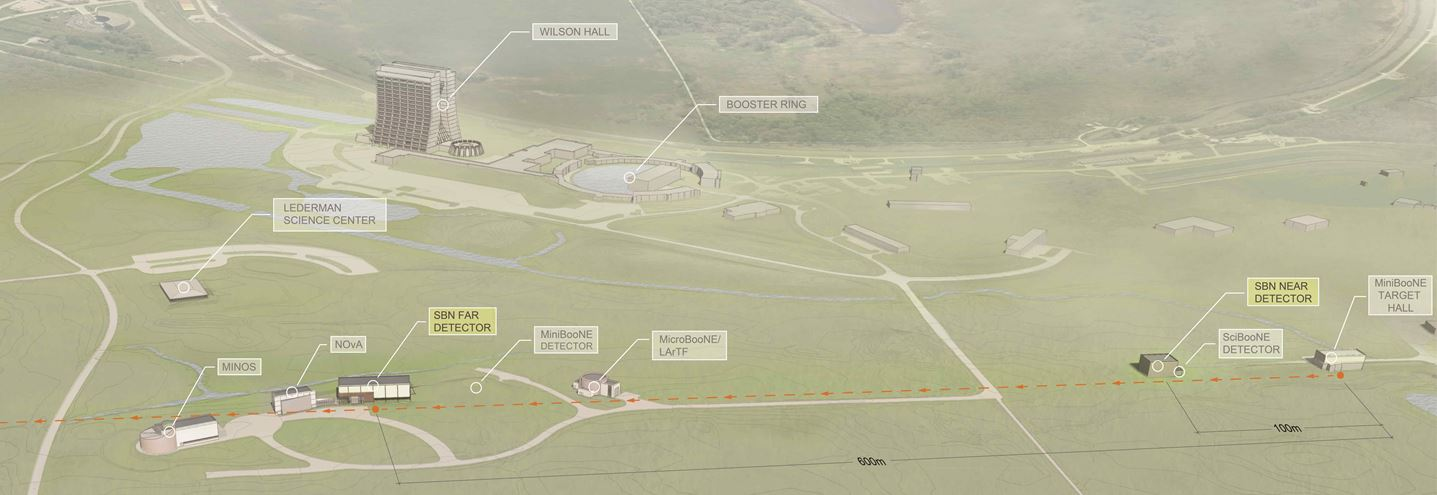
\includegraphics[width=\textwidth]{sbn_figures/SBN_Map.jpeg}
  \caption[SBN Detector Locations]{An aerial view of the SBN program.  The three detectors are highlighted in yellow, and (from right to left, along the path of the beam) are \sbnd, \uboone, and \icarus}
  \label{fig:sbn_birdseyeview}
\end{figure}

\section{Physics Program}

The Short Baseline Neutrino program has an aggressive agenda to probe anomalous oscillation signals, and to follow up on \uboone's Low Energy Excess analysis.  It's worth noting that \nue appearance is not the only physics analysis that will be performed by the SBN Program.  This thesis will focus on \nue appearance, however to resolve questions of sterile neutrinos the SBN program will also have to observe:

\begin{itemize}

\item {\bf \numu Disapperance}  As mentioned above, the channels of \nue appearance and \numu disappearance are intricately connected in models of sterile neutrino oscillations.  So, for any measurement of \nue appearance at the SBN Program to be interpreted in a 3+1 model of oscillations, it should be accompanied by an amount of \numu disappearance consistent with the level of \nue appearance.  Much more about \numu disappearance is available in the SBN Program Proposal \cite{Antonello:2015lea} 

\item {\bf Neutral Current Disappearance (Active flavor Disapperance)}  Just as the \nue and \numu oscillation signals are connected if a sterile neutrino is present, the total active flavor content of the beam (\nue + \numu + \nutau) should be modulated by the presence of a sterile neutrino in a consistent way.  \lartpc technology allows measurement of the total neutral current interaction rate using channels such as Neutral Current $\pi^0$ production.

\end{itemize}

Also of interest is the suite of cross section measurements that the SBN Program can perform, particularly with the SBND experiment (the near detector).  In the event that \uboone observes the \MB anomaly to be an unexpected beam background or cross section, SBND can probe this result with nearly two orders of magnitude faster collection of events than \uboone.

\section{Simulation and Monte Carlo Predictions of Event rates}

For the calculation and study of the physics sensitivity of the Short Baseline Program, a Monte Carlo Simulation predicts the event rate at each detector in the beamline.  The procedure of the simulation is:

\begin{enumerate}

  \item {\bf Booster Beam Monte Carlo} The first stage in the simulation is the Monte Carlo simulation of the Booster Neutrino Beam production. This is a geant4 based simulation that follows 8 GeV protons through interactions on the BNB beryllium target. The hadrons produced in the interaction are focus by the horn and decay, in flight, to neutrinos, which are then propagated to a window in front of a detector. It is at this stage of the simulation that we include a series of reweighting variables for each neutrino to estimate the systematic uncertainty on the flux at each detector, as well as the correlations between detectors (additional information in Section~\ref{section:flux_uncert}).

  \item {\bf \textsc{Genie} Neutrino Interactions} The output of the beam Monte Carlo is a file of neutrinos at the detector containing information about the flavor, momentum, and position, as well as the parentage from the beam source, for each neutrino. The interactions of these neutrinos are simulated with the genie software which outputs a series of particles exiting the argon nucleus \cite{Andreopoulos:2009rq}. 

  \item {\bf \textsc{Geant4} Simulation of Particles} The particles which exit the argon nucleus, as generated by genie, are then propagated through the liquid argon using a \textsc{Geant} \cite{Agostinelli:2002hh} simulation built in to the LArSoft framework \cite{Church:2013hea}. In particular this helps estimate the containment of electromagnetic showers, interaction location of photons from \pizero production and $\Delta$ resonances, as well as containment of minimally ionizing particles such as muons and charged pions.

  \item {\bf Monte Carlo Truth Based Information}  After the geant simulation of the neutrino interaction we extract the event information using the Monte Carlo truth information. Estimated reconstruction efficiencies and energy resolutions are applied at this stage, as well as simulated event selections based on expected detector performance.  See Section~\ref{subsection:event_reco} for more detail.

\end{enumerate}


\subsection{Background Classification}

For the study of the Short Baseline Neutrino Program's sensitivity to anomalous appearance of electron neutrinos, it is essential to have a comprehensive estimate of the various backgrounds with realistic distributions based on expected reconstruction ability.  Primarily, the \nue appearance background consists of 3 broad categories: intrinsic \nue's from the beam, mis-identified electromagnetic showers produced by the beam (primarily from \numu), and cosmic induced backgrounds coincidental with the beam spill.

\begin{enumerate}

  \item {\bf Intrinsic \nue } - the Booster Beam, while primarily composed of muon neutrinos, has contamination of electron neutrinos that account for about 0.5\% of the beam.  While this is a small contamination, it is the same order of magnitude as the best fit oscillation parameters for possible sterile neutrino hints. This means that, compared to any possible signal, the intrinsic electron neutrinos in the beam are a large background and must be carefully quantified.  An 80\% reconstruction efficiency is applied to these events, and an electromagnetic shower energy of 200MeV is set as a threshold for event selection.  This is to ensure good selection and reconstruction in the data, and has a moderate impact at lower energies on the efficiency (~30\% loss in the 200 to 350 MeV bin) with small impacts (~5\%) at higher energies.



  \item {\bf Neutral Current Photon Misidentification} - The photons produced in the detector by neutral current processes can produce an electromagnetic shower similar to electron neutrinos.  An example of a reaction that produces high energy photons is an interaction with neutral pions in the final state, as well as radiative decays from nucleon resonances. It's expected that, without cuts, these backgrounds can be large and in the same energy region as a signal search. However, analysis cuts can greatly reduce this background.

  \begin{enumerate}

    \item{\em Two photon cut:} In an event with candidate electromagnetic showers, the presence of multiple showers indicates there could be neutral pion production in the neutrino interaction.  See, for example, Figure~\ref{fig:argo_pi0} for an ArgoNeuT event with multiple showers.  For this analysis, if a second found is found with energy greater than 100 MeV, the event is rejected from the electron neutrino sample.  The energy cut, 100 MeV, is lower than the threshold for candidate electron showers because the second photon does not need accurate reconstruction, it just needs to be identified.

    \item{\em Photon Conversion Gap:} In events where the neutrino interaction produces high energy photons, it can at times also product hadronic activity at the vertex.  If more than 50 MeV of energy is observed at the vertex, and a gap between the electromagnetic shower and the vertex is detected with more than 3 centimeters (in \uboone, this is up to 30 wires), the event is rejected.

    \item{\em dE/dx Cut:} In this study, for events passing the previous two cuts, and 94\% rejection was applied.  This accounts for the expected resolution, in the SBN detectors, of the calorimetric based cut on the ionization of the first few centimeters of a shower.  For more about the power of the dE/dx cut in data, see Section~\ref{sec:argo_dedx}

  \end{enumerate}


  \item {\bf Neutrino Electron Scattering}  - neutrinos can scatter off both the nucleus and the orbiting electrons in an atom. An interaction off an electron ejects the electron at high energy. Experimentally, the signature of this interaction is a very forward going electron and nothing else in the event, which mimics a \nue charged current interaction. Fortunately, these events have a very low interaction rate compared to scattering off of a nucleus and are a secondary background.  The forward angle and relatively high energy also make them a removable background.

  \item {\bf \numu Charge Current Misidentification} - The last item considered as a possible background are misidentified charged current interactions from muon neutrinos. The rate at which this happens is poorly know and needs to be measured, but there are some scenarios that could lead to this occurring. For example, in an event near the boundary of the TPC where a \pizero is produced along with the primary muon, if the muon exits and one photon converts outside the TPC there will be one electromagnetic shower seen and the track of the muon will be impossible to tag as a muon or charged pion. Though somewhat contrived, this example only serves to illustrate that this background should be considered. Here, events are included from \numu CC interactions if there is a single photon in the detector and the primary muon exits with less than one meter in the detector.
  
  \item {\bf Cosmic Photons} - Cosmic induced photons in the TPC have the potential to be incorrectly tagged as electrons. This is a background that will be very tightly constrained from off-beam backgrounds, but estimates from simulation are included here.

  \item{\bf ``Dirt'' Events} - Neutrinos can interact with the material surrounding the active volume of the detector as well.  Though this is not, strictly speak, ``dirt'', events where detector external neutrino interactions travel into the TPC and deposit energy can cause a background to the \nue appearance analysis.  In particular, photon production external to the TPC can generate a high energy photon that travels into the TPC and doesn't ionize the argon until it has entered the TPC for some distance.  This background will be constrained with both simulation and data, however, preliminary estimates are included.  Additionally, strong cuts can be made with fiducial volumes.

\end{enumerate}

\begin{figure}[htbp]
  \centering
  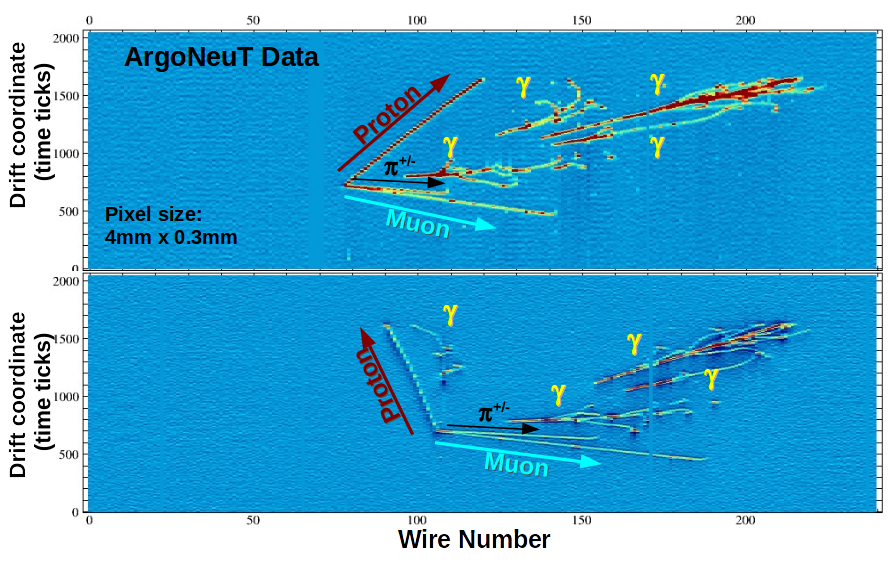
\includegraphics[width=0.95\textwidth]{sbn_figures/ArgoNeuT_Labels.png}
  \caption{caption}
  \label{fig:argo_pi0}
\end{figure}

\subsection{Simulated Event Reconstruction and Analysis cuts}
\label{subsection:event_reco}

In order to perform the best estimate of the physics sensitivity of the SBN program, an estimate of reconstruction effects must be incorporated into the event rates.  Additionally, some analysis cuts to reduce cosmic and ``dirt'' events are included.

The simplest cut is the fiducial volume cut applied in all three detectors.  Events with a vertex found to be outside of the fiducial volume are rejected, and the volume is set as:
\begin{itemize}
\item{\bf X:} The drift direction has a cut of 25cm from each edge, which reduces ``dirt'' backgrounds significantly.
\item{\bf Y:} The vertical direction also has a cut of 25cm from each edge, which reduces ``dirt'' backgrounds significantly.
\item{\bf Z:} The beam direction has an upstream cut of 30cm, to reject events that are entering the detector from the front.  There is a downstream cut of 50cm to aid in detection of electromagnetic showers.
\end{itemize}

To simulate calorimetric energy reconstruction, the incoming neutrino energy in each Monte Carlo event is estimated by summing the energy of the lepton (or the $\gamma$ the faking an electron) and all charged hadrons above observation thresholds present in the final state.  The observation thresholds are defined by requiring that the kinetic energy of each hadron be sufficient that it cross at least 2 wires, and are guided by \argoneut data.  For protons, for example, the threshold is 20 MeV. 

The event rate distributions, and the tables of event rates, are shown in Figure~\ref{fig:sbn_event_rates_no_signal} and sidewaysTable~\ref{tab:sbn_event_rates_no_signal}.

\begin{figure}[htbp]
    \centering
    \begin{subfigure}[]{0.49\textwidth}
        \centering
        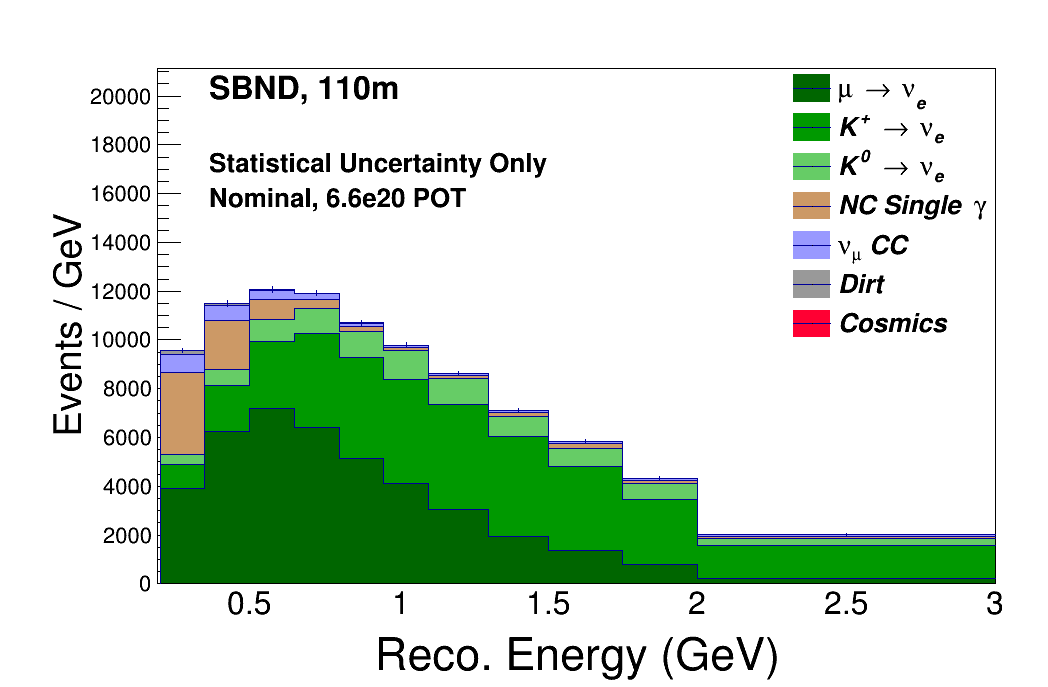
\includegraphics[width=\textwidth]{sbn_figures/nominal_nue_appearance_nosig_SBND_110m}
    \end{subfigure}
    ~
    \begin{subfigure}[]{0.49\textwidth}
        \centering
        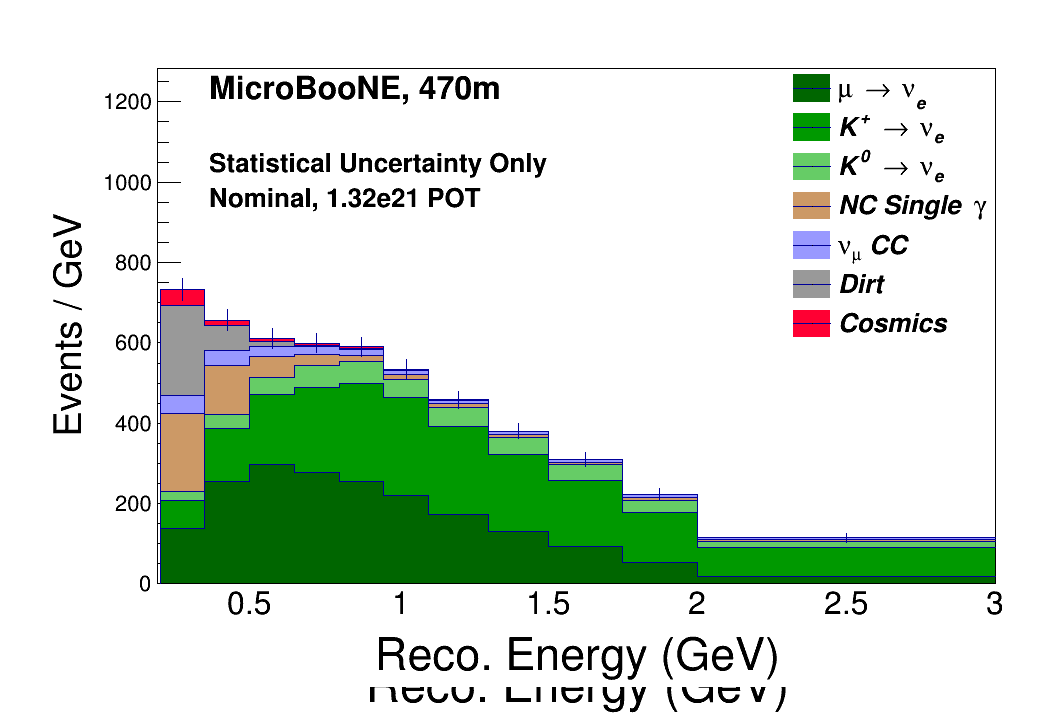
\includegraphics[width=\textwidth]{sbn_figures/nominal_nue_appearance_nosig_MicroBooNE_470m}
    \end{subfigure}
    \\
    \begin{subfigure}[]{0.49\textwidth}
        \centering
        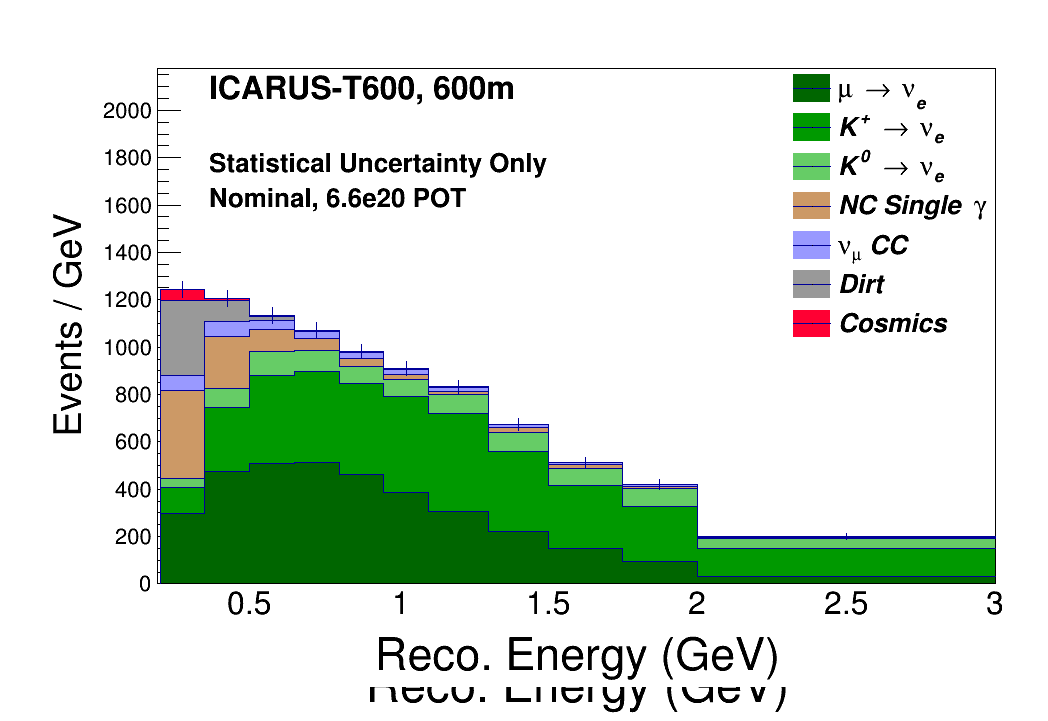
\includegraphics[width=\textwidth]{sbn_figures/nominal_nue_appearance_nosig_ICARUS-T600_600m}
    \end{subfigure}
    \caption[SBN Event Rates]{The predicted event rates for the SBN program in all three detectors, assuming 2.2e20 Protons on Target delivered each year.  For this analysis, \uboone is assumed to have 6 years of running (its original 3 + 3 with the SBN program)}.
   \label{fig:sbn_event_rates_no_signal}
\end{figure}

\section{Simulation of an Oscillation Signal}

To predict a sensitivity of an experimental program, a model must be used to generate a sample of events that are signal events.  In this case, as mentioned in Section~\ref{sec:global_fits}, the two neutrino oscillation probability formula is used to transmute muon neutrinos into electron neutrinos.  While the 3+1 model is not the only viable or interesting method to simulate a signal, it is the most straightforward to compare to other experiments.  

To build a signal sample, a ``fully oscillated'' sample of Monte Carlo is generated where every \numu has been changed to a \nue, and then the sample of \nue's is propagated through the GENIE event generator and the rest of the simulation.  Each electron neutrino, formerly muon neutrino, is ``reconstructed'' in the same manner as the electron neutrino candidates in the background sample, with identical cuts.  

Later, a sensitivity curve will be shown as a function of ($\Delta_m^2,\text{sin}^2 2 \theta$).  This refers to physical parameters of neutrino oscillation, where $\Delta m^2$ is the mass splitting, squared, between known neutrinos and a supposed sterile state.  Sin${}^2 2 \theta$ represents the amplitude of the oscillation and is a combination of matrix elements from the neutrino mixing matrix above.  For a fixed pair of ($\Delta_m^2,\text{sin}^2 2 \theta$), each transmuted electron neutrino in the ``fully oscillated'' sample is scaled according to the formula 

\begin{equation}
% \centering
P(\numu \rightarrow \nue) = sin^2(2 \theta_{\mu e})\times sin(1.27 \frac{\Delta m^2 L}{E} \frac{[eV^2][m]}{[MeV]})),
\end{equation}
where L and E are known from the Monte Carlo as the distance the neutrino has traveled since the decay of it's parent particle, and the true energy of the neutrino.  Because the neutrino beam is broad band, peaked near 1 GeV but with substantial flux down to several hundred MeV and out to 3 GeV, the oscillation probabilities at each detector are smeared and the predicted signal can cover a broad spectrum of neutrino energies (see Figure~\ref{fig:osc_prob} )
% tables were made with the help of http://www.tablesgenerator.com/

\begin{figure}[htbp]
  \centering
  \includegraphics[width=\textwidth]{sbn_figures/osc_prob.pdf}
  \caption[BNB Oscillation Probability]{Oscillation Probability bands as a function of distance from the proton target for the SBN program.  Shown are the bands for two of the global best fit results.}
  \label{fig:osc_prob}
\end{figure}


\begin{sidewaystable}[htbp]
\centering

\caption{Background Rates, broken out by analysis bin and origin, for the SBND experiment for 6.6e20 POT. The signal is from the Giunti {\em et al.} best fit point}
\label{tab:sbn_event_rates_no_signal}
\begin{tabular}{r|cccccccccll}
\multicolumn{1}{l|}{Bins [GeV]} & \multicolumn{1}{l}{$\mu\rightarrow\nu_e$} & \multicolumn{1}{l}{$K^{\pm}\rightarrow \nu_e$} & \multicolumn{1}{l}{$K^0 \rightarrow \nue$} & \multicolumn{1}{l}{$\nu + e^-$} & \multicolumn{1}{l}{NC~$\pi^0$} & \multicolumn{1}{l}{$\Delta \rightarrow N\gamma$} & \multicolumn{1}{l}{$\nu_{\mu}$~CC} & \multicolumn{1}{l}{Dirt} & \multicolumn{1}{l}{Cosmic} & Signal               & Total \\ \hline
\textbf{0.20-0.35}    & 45                          & 16                          & 6                           & 3                        & 56                         & 0                          & 10                         & 47                       & 7                          & 13                   & 189   \\
\textbf{0.35-0.50}    & 71                          & 40                          & 12                          & 5                        & 33                         & 1                          & 10                         & 13                       & 1                          & 28                   & 186   \\
\textbf{0.50-0.65}    & 76                          & 56                          & 15                          & 5                        & 14                         & 2                          & 6                          & 3                        & 1                          & 64                   & 176   \\
\textbf{0.65-0.80}    & 77                          & 57                          & 14                          & 7                        & 8                          & 2                          & 4                          & 1                        & 0                          & 82                   & 169   \\
\textbf{0.80-0.95}    & 69                          & 58                          & 11                          & 9                        & 5                          & 2                          & 4                          & 1                        & 0                          & 73                   & 157   \\
\textbf{0.95-1.10}    & 58                          & 61                          & 11                          & 5                        & 3                          & 1                          & 3                          & 0                        & 0                          & 57                   & 142   \\
\textbf{1.10-1.30}    & 61                          & 82                          & 16                          & 3                        & 3                          & 1                          & 3                          & 0                        & 0                          & 48                   & 170   \\
\textbf{1.30-1.50}    & 44                          & 67                          & 17                          & 1                        & 4                          & 0                          & 3                          & 0                        & 0                          & 25                   & 136   \\
\textbf{1.50-1.75}    & 37                          & 67                          & 18                          & 1                        & 4                          & 0                          & 2                          & 0                        & 0                          & 13                   & 129   \\
\textbf{1.75-2.00}    & 24                          & 58                          & 19                          & 1                        & 2                          & 0                          & 2                          & 0                        & 0                          & 5                    & 106   \\
\textbf{2.00-3.00}    & 30                          & 121                         & 39                          & 1                        & 5                          & 0                          & 4                          & 0                        & 0                          & 4                    & 201   \\ \hline
Total                 & 593                         & 684                         & 177                         & 39                       & 137                        & 8                          & 50                         & 65                       & 10                         & \multicolumn{1}{c}{} &      
\end{tabular}
\end{sidewaystable}


\begin{sidewaystable}[htbp]
\centering

\caption{Background Rates, broken out by analysis bin and origin, for the \uboone experiment for 6.6e20 POT. The signal is from the Giunti {\em et al.} best fit point}
\begin{tabular}{r|cccccccccll}
\multicolumn{1}{l|}{Bins [GeV]} & \multicolumn{1}{l}{$\mu\rightarrow\nu_e$} & \multicolumn{1}{l}{$K^{\pm}\rightarrow \nu_e$} & \multicolumn{1}{l}{$K^0 \rightarrow \nue$} & \multicolumn{1}{l}{$\nu + e^-$} & \multicolumn{1}{l}{NC~$\pi^0$} & \multicolumn{1}{l}{$\Delta \rightarrow N\gamma$} & \multicolumn{1}{l}{$\nu_{\mu}$~CC} & \multicolumn{1}{l}{Dirt} & \multicolumn{1}{l}{Cosmic} & Signal & Total \\ \hline
\textbf{0.20-0.35}        & 21                          & 10                          & 4                           & 3                        & 29                         & 0                          & 7                          & 34                       & 6                          & 2      & 113   \\
\textbf{0.35-0.50}        & 38                          & 20                          & 6                           & 2                        & 18                         & 1                          & 6                          & 9                        & 2                          & 10     & 101   \\
\textbf{0.50-0.65}        & 45                          & 26                          & 6                           & 2                        & 8                          & 1                          & 4                          & 2                        & 1                          & 16     & 94    \\
\textbf{0.65-0.80}        & 42                          & 32                          & 8                           & 1                        & 4                          & 1                          & 3                          & 0                        & 1                          & 16     & 92    \\
\textbf{0.80-0.95}        & 38                          & 36                          & 8                           & 1                        & 2                          & 1                          & 2                          & 0                        & 0                          & 12     & 90    \\
\textbf{0.95-1.10}        & 33                          & 37                          & 7                           & 0                        & 2                          & 0                          & 2                          & 0                        & 0                          & 9      & 81    \\
\textbf{1.10-1.30}        & 35                          & 44                          & 9                           & 0                        & 2                          & 0                          & 2                          & 0                        & 0                          & 7      & 92    \\
\textbf{1.30-1.50}        & 26                          & 38                          & 9                           & 0                        & 1                          & 0                          & 2                          & 0                        & 0                          & 4      & 76    \\
\textbf{1.50-1.75}        & 23                          & 41                          & 10                          & 0                        & 2                          & 0                          & 2                          & 0                        & 0                          & 2      & 78    \\
\textbf{1.75-2.00}        & 14                          & 31                          & 8                           & 0                        & 2                          & 0                          & 2                          & 0                        & 0                          & 1      & 56    \\
\textbf{2.00-3.00}        & 18                          & 72                          & 17                          & 0                        & 5                          & 0                          & 4                          & 0                        & 0                          & 1      & 115   \\ \hline
Total                     & 331                         & 388                         & 91                          & 10                       & 75                         & 5                          & 34                         & 46                       & 11                         &        &      
\end{tabular}
\end{sidewaystable}

\begin{sidewaystable}[htbp]
% \begin{adjustbox}{width=q\textwidth}{
\centering

\caption{Background Rates, broken out by analysis bin and origin, for the \icarus experiment for 6.6e20 POT. The signal is from the Giunti {\em et al.} best fit point}
\begin{tabular}{r|cccccccccll}
\multicolumn{1}{l|}{Bins [Gev]} & \multicolumn{1}{l}{$\mu\rightarrow\nu_e$} & \multicolumn{1}{l}{$K^{\pm}\rightarrow \nu_e$} & \multicolumn{1}{l}{$K^0 \rightarrow \nue$} & \multicolumn{1}{l}{$\nu + e^-$} & \multicolumn{1}{l}{NC~$\pi^0$} & \multicolumn{1}{l}{$\Delta \rightarrow N\gamma$} & \multicolumn{1}{l}{$\nu_{\mu}$~CC} & \multicolumn{1}{l}{Dirt} & \multicolumn{1}{l}{Cosmic} & Signal & Total \\ \hline
\textbf{0.20-0.35}        & 585                         & 151                         & 59                          & 59                       & 504                        & 1                          & 112                        & 23                       & 3                          & 62     & 1496  \\
\textbf{0.35-0.50}        & 938                         & 282                         & 99                          & 137                      & 299                        & 13                         & 95                         & 10                       & 1                          & 81     & 1874  \\
\textbf{0.50-0.65}        & 1076                        & 417                         & 134                         & 20                       & 120                        & 21                         & 58                         & 5                        & 0                          & 58     & 1851  \\
\textbf{0.65-0.80}        & 961                         & 579                         & 155                         & 19                       & 54                         & 23                         & 37                         & 2                        & 0                          & 41     & 1831  \\
\textbf{0.80-0.95}        & 769                         & 622                         & 158                         & 32                       & 33                         & 13                         & 22                         & 1                        & 0                          & 24     & 1651  \\
\textbf{0.95-1.10}        & 619                         & 641                         & 172                         & 51                       & 22                         & 7                          & 14                         & 1                        & 0                          & 14     & 1528  \\
\textbf{1.10-1.30}        & 607                         & 866                         & 210                         & 32                       & 28                         & 4                          & 13                         & 1                        & 0                          & 9      & 1761  \\
\textbf{1.30-1.50}        & 391                         & 817                         & 167                         & 26                       & 33                         & 1                          & 12                         & 1                        & 0                          & 4      & 1449  \\
\textbf{1.50-1.75}        & 339                         & 864                         & 186                         & 7                        & 51                         & 1                          & 21                         & 0                        & 0                          & 2      & 1468  \\
\textbf{1.75-2.00}        & 203                         & 660                         & 168                         & 0                        & 25                         & 0                          & 25                         & 0                        & 0                          & 1      & 1083  \\
\textbf{2.00-3.00}        & 231                         & 1360                        & 267                         & 7                        & 84                         & 1                          & 77                         & 0                        & 0                          & 1      & 2026  \\ \hline
Total                     & 6721                        & 7260                        & 1776                        & 389                      & 1252                       & 86                         & 486                        & 44                       & 5                          &        &      
\end{tabular}
% \end{adjustbox}
\end{sidewaystable}





\chapter{Systematic Uncertainties in the Short Baseline Neutrino Program}
\label{chp:systematics}

In the previous chapter, the motivation for the Fermilab Short Baseline Neutrino program was presented and the expected event rates were shown, as well as the methods of calculating an expected signal from a 3+1 model.  However, the most detailed simulation (or data analysis, for that matter) is not consequential without a robust calculation of systematic uncertainties.

In this chapter, the systematic uncertainties for the Short Baseline are discussed.  Of particular importance are the uncertainties from the flux and neutrino interactions.  The flux for the Booster Neutrino Beam, while among the best known neutrino beam fluxes, still has residual uncertainties of up to 15\% \cite{AguilarArevalo:2008yp}.  Similarly, the uncertainty in the model of neutrino interactions has a 10 to 15\% normalization uncertainty for the quasi-elastic and resonant events that are most important to the oscillation searches.  Considering that the amplitude of any sterile neutrino oscillation effect is very small, with oscillation probabilities that peak at 1\% or less, constraining the systematic uncertainties in the Short Baseline Program is absolutely essential.

The strength of the Short Baseline Program's oscillation search comes, ultimately, from two factors:  the \lartpc technology allows excellent event identification and background rejections, and the near detector, SBND, allows for large cancellation of systematic uncertainties.  In this chapter, the method for quantifying the cancellation of systematic uncertainties is presented.


\section{General Framework for quantification of uncertainties}

\label{sec:multi_weight}

In this analysis, the uncertainties that matter are the systematic uncertainties on the final distribution of event rates.  Since the goal is to produce a sensitivity calculation for an expected signal, the numerical value of the sensitivity can be calculated with a $\chi^2$ calculation:

\begin{equation}
\begin{centering}
\label{eq:chi_sq}
\chi^2(\Delta m^2, \text{sin}^2 2 \theta ) = \sum_{i,j} [N^{null}_i - N^{osc}_i(\Delta m^2, \text{sin}^2 2 \theta ) ] \times E^{-1}_{i,j} \times [N^{null}_j - N^{osc}_j(\Delta m^2, \text{sin}^2 2 \theta ) ],
\end{centering}
\end{equation}

where $N^{null}_i$ is the expected event rate in the $i^{th}$ analysis bin with no oscillation signal, and $N^{osc}_i(\Delta m^2, \text{sin}^2 2 \theta )$ is the expected event rate in the $i^{th}$ analysis bin if there is an oscillation signal from a 3+1 model with the specified mass splitting and amplitude.  In the \nue appearance analysis, this is simplified to 
\begin{equation}
\begin{centering}
N^{null}_i - N^{osc}_i(\Delta m^2, \text{sin}^2 2 \theta ) = S_i(\Delta m^2, \text{sin}^2 2 \theta )
\end{centering}
\end{equation}
where S is the expected signal events from the specified parameters in the $i^{th}$ bin.

$E_{i,j}$ in the $\chi^2$ computation is the covariance matrix, a statistical tool to encode correlated uncertainties.  In practice, the computation of the covariance matrix is the most challenging aspect of the $\chi^2$ calculation because it requires careful determination of how the uncertainties under study are correlated.  For this work, the correlations of uncertainties are quantified with the ``multiple universe'' method \footnote{Nothing to do with the cosmological idea of the multiverse}.  Much more will be said about the computation and use of the covariance matrix in Section~\ref{sec:covariance_matrix}.

\subsection{Multiple Universe Error Propagation and Reweighing methods}

In a complex chain of simulation and analysis such as a prediction of event rates in a neutrino detector, it can be challenging to understand the effect of, for example, an uncertainty of hadron production at the proton target on the final distribution of neutrino events in the detector.  Some intuitive knowledge is of course present: if the amount of neutrino producing particles generated at the target by proton interactions is under (or over) estimated, the event rates in the final analysis distribution at the detector will also be under (over) estimated.  To precisely quantify the relationship between initial variable underlying the simulation and the final distributions of events, a reweighing scheme with multiple universes is used.

\subsubsection{Reweighing Events}

The the models used in the Monte Carlo simulations of neutrino experiments, there is always a class of parameters that feed the models and simulations:  the neutrino cross sections dictate how many events appear in the detector; the hadron interaction cross section dictates both the amount and variation of hadrons produced in the beam target.  These broad examples are meant to highlight that the Monte Carlo must be based upon not just a physics model but the input parameters to that model.  In the case of hadron production when the protons interact with the target, an assumption must be made about the cross section of that interaction.  While the Monte Carlo is naturally based on the best estimate of the input parameters, it's insufficient to estimate the uncertainty in the simulation without using the uncertainty on the input parameters.

As a concrete example, the beam simulation (originally developed by the \MB collaboration) for the Booster Neutrino Beam uses the Sangford-Wang parameterization to model the double differential pion production cross section for secondary particles at the target.  The parameterization, 

\begin{equation}
\begin{centering}
\frac{d^2 \sigma}{dp d\Omega}(p,\theta) = c_1 \left(1 - \frac{p}{p_B - c_9}\right)\text{exp}\left(- c_3 \frac{p^{c_4}}{p^{c_5}_B} - c_6 \theta (p - c_7 p_B \text{cos}^{c_8}\theta) \right),
\end{centering}
\end{equation}

is a complicated system with eight free parameters which have been fit against data from the HARP and BNL E901 experiments.  The parameters are also not independent, but instead can have strong correlations.  The knowledge of these parameters is not perfect, and indeed the best fit parameters have imperfect agreement with data (see Figure~\ref{fig:sanford_wang_harp}).  However, the fact that the parameters are correlated allows some freedom to change the fit parameters such that the overall parameterization remains consistent with data.  When the parameters are changed from the nominal value to a different, consistent parameterization, it is a different ``Universe'' for this set of parameters.  It's worth noting that the variation in the cross section that comes about by varying the paremeters is the source of the dashed bands in Figure~\ref{fig:sanford_wang_harp}.

In general, varying underlying physical parameters to a model produces a new result.  Unfortunately, Monte Carlo simulation of neutrino beams and interactions is computationally expensive, and repeating the simulation for every variance of a parameter is not possible.  In this case, a `reweighting scheme' is used.  For the moment, assume in a particular universe the Sanford-Wang parameterization above has been increased by a factor $X$ for a particular neutrino in the simulation.  Rather than reproduce this neutrino, in the computation of the final event distributions the same event is used in the same energy bin, but is given a relative weight of $1 + X$.  This factor can be recomputed for every neutrino that is in the final distribution, leading to an event rate distribution that would have been found if the entire simulation were repeated.

In general, this method of `reweighting' applies new weights to every neutrino in the final analysis for each ``Universe.''  By varying the underlying parameters (in a way that leaves them consistent with constraining data) of a physical model many times, a large sample of universes is obtained, and the event distributions can be computed in each universe.  The parameters, however, can not be tweaked completely at random and instead must be drawn according to a Gaussian distribution (if a single uncertainty) or through more complicated methods if a series of correlated parameters.  \MB, for example, varies the Sanford-Wang parameters together through the Cholesky method.


\begin{figure}[tb]
  \centering
  \includegraphics[width=\textwidth]{systematics_figures/sanford_wang_harp}
  \caption[HARP Data and Sanford-Wang Fit]{The HARP Data (points), and the Sanford-Wang best fit parameterization (solid line).  The dashed lines represent a 68\% uncertainty band on the parameterization model from varying the fit parameters within their correlated uncertainties.  The Figure from \cite{AguilarArevalo:2008yp}.}
  \label{fig:sanford_wang_harp}
\end{figure}

\section{Determination of Covariance Matrices}
\label{sec:covariance_matrix}

Using the methods described above for applying weights on an event-by-event basis, it's possible to generate a suite of ``Universes'' of event rate histograms, where the value of each analysis bin can be known in each universe as $N^i_{\text{Univ.} m}.$  In this document, since there are three detectors under consideration, the vector of event rates in each analysis bin, $N$, is a concatenation of the vector of event rates in each detector.  If there are $P$ total analysis bins in each detector, then 
\begin{multline}
\vec{N}_{\text{Nom.}} = (~N_{\text{Nom.}}^{1,~SBND},~\dots, ~N_{\text{Nom.}}^{P,~SBND},~N_{\text{Nom.}}^{1,~\uboone}, \\ 
\dots,N_{\text{Nom.}}^{P,~\uboone},~N_{\text{Nom.}}^{1,~\icarus},~\dots~N_{\text{Nom.}}^{P,~\icarus} ~)
\end{multline}
and in each universe where an underlying physical parameter has been varied:
\begin{multline}
\vec{N}_{\text{Univ.}~m} = (~N_{\text{Univ.}~m}^{1,~SBND},~\dots~N_{\text{Univ.}~m}^{P,~SBND},~N_{\text{Univ.}~m}^{1,~\uboone}, \\
\dots,~N_{\text{Univ.}~m}^{P,~\uboone},~N_{\text{Univ.}~m}^{1,~\icarus}~\dots~N_{\text{Univ.}~m}^{P,~\icarus} ~).
\end{multline}

With these vectors, it's possible to calculate deviation from the nominal values due to the underlying uncertainties in an analysis bin:
\begin{equation}
\begin{centering}
\sigma^i = \sqrt{\frac{1}{M}\sum_{\text{All Univ.}~m}^{M} \left( N^i_{\text{Nom.}} - N^i_{\text{Univ.~m}}\right)^2}
\end{centering}
\label{eq:bin_uncert}
\end{equation}

This measurement of the uncertainty in this way gives an estimate of the uncertainty in single detector experiments, where bin to bin correlations are ignored.  In other words, $\sigma^i$ is the uncertainty in the $i^{th}$ analysis bin when the existence of all the other bins, in any detector, are ignored.  See Figures~\ref{fig:sys_flux_uncert_fracUncert}, \ref{fig:sys_xsec_uncert_fracUncert} for this measurement due to flux and cross section uncertainties, below.  In a practical sense, this measurement of the uncertainty is not useful for the computation of sensitivities or significances of a signal, but only provides an easily interpreted measure of the uncertainty of a single detector experiment.

A more useful statical tool is the covariance matrix, $E$, defined at each bin as
\begin{equation}
\begin{centering}
E^{i,j} = \frac{1}{M}\sum_{\text{All Univ.}~m}^{M} \left[ N^i_{\text{Nom.}} - N^i_{\text{Univ.~m}}\right] \times \left[ N^j_{\text{Nom.}} - N^j_{\text{Univ.~m}}\right].
\end{centering}
\label{eq:cov_mat}
\end{equation}

Covariance matrices that arise from uncertainty sources that are uncorrelated are separable, in the sense that for a complete analysis the final covariance matrix can be constructed as the sum of the matrices from each source.  In this analysis, a covariance matrix is calculated for the flux and cross section uncertainties for beam intrinsic events, and the matrix is estimated for the backgrounds from ``Dirt'' and cosmic induced events, as well as detector systematics.
\begin{equation}
\begin{centering}
\label{eq:tot_cov_mat}
E = E_{\text{Stat.}} + E_{\text{Flux}} + E_{\text{Cross Section}} + E_{\text{Dirt}} + E_{\text{Cosmic}} + E_{\text{Det. Syst.}}
\end{centering}
\end{equation}

The covariance matrix is more easily visualized in the form of some of it's transforms, the fractional covariance matrix
\begin{equation}
\begin{centering}
F^{i,j} \equiv \frac{E^{i,j}}{N^{i} N^{j}}
\end{centering}
\end{equation}
and the correlation matrix
\begin{equation}
\begin{centering}
C^{i,j} \equiv \frac{ E^{i,j} }{ \sqrt{E^{i,i}} \sqrt{E^{j,j}} }.
\end{centering}
\end{equation}

See Figures~\ref{fig:syst_flux_fracmatrix}, \ref{fig:syst_xsec_fracmatrix} for examples of the fractional covariance matrix, and Figures~\ref{fig:syst_flux_corrmatrix}, \ref{fig:syst_xsec_corrmatrix} for examples of the correlation matrix.  The fractional error matrix shows which analysis bins have the largest systematic uncertainty, though because it is relative it can be deceiving: bins with high systematic uncertainties might not be important bins in the analysis. 

The correlation matrix is an excellent visualization of the power of the covariance matrix technique.  It is limited to between -1 (full anticorrelation) and 1 (full correlation), and each entry at bin $(i,j)$ displays how correlated the $i^{th}$ bin is to the $j^{th}$ bin.  This is the vital information that allows correlated uncertainties in a multi detector experiment to cancel: a deviation at the far detector becomes significant (even if it is within the nominal uncertainty at that bin given by Eq. \ref{eq:bin_uncert}) if the deviation is not seen at a near detector {\bf and} the correlation between near and far is large.  The correlation matrices show the magnitude of exactly that correlation, while the covariance matrix (\ref{eq:cov_mat}) is the mathematical tool that carries correlation information to the $\chi^2$ calculation.


\section{Uncertainties from Neutrino Flux}

\label{section:flux_uncert}

As might be expected, the neutrino flux is highly correlated across the three detectors in the Booster Neutrino Beam.  However, the exact shape of the flux is not identical, especially at the near detector.  Figure~ \ref{fig:sbn_flux} shows the flux at the three detectors.

\begin{figure}[htbp]
  \centering
  \includegraphics[width=0.45\textwidth]{sbn_figures/bnb_flux_nu_100m.eps}
  \includegraphics[width=0.45\textwidth]{sbn_figures/bnb_flux_nu_470m.eps}
  \includegraphics[width=0.45\textwidth]{sbn_figures/bnb_flux_nu_700m.eps}
  \caption[BNB Fluxes]{The neutrino flux from the Booster Beam at the three locations of the SBN Program.  The flux falls at approximately $1/r^2$, however, the near detector sees a non-pointlike source due to its proximity to the decay pipe.}
  \label{fig:sbn_flux}
\end{figure}

The covariance matrix for the uncertainties from the neutrino flux is built, as described above, using a multi universe approach.  As alluded to in Table~\ref{tab:mb_flux_uncert}, the uncertainties from the neutrino flux are well quantified by \MB.  However, their uncertainty calculations concerned a single detector, while the SBN Program is a multi detector experiment.  To properly quantify the correlated uncertainties between the three detectors, the flux at each detector has to be varied (using the multiple universe reweighting scheme above) consistently: in the $N^{th}$ Universe, the underlying physical parameters that have been changed are changed identically in all three detectors.  The event distributions can be calculated again in each universe, for all three detectors, and from them the covariance distribution is built for the flux uncertainties.

For the results shown here, the following uncertainties are considered in the computation of the flux covariance matrix:

\begin{itemize}
\item Primary production of $\pi^+$ , $\pi^-$ , $K^+$ , $K^−$ , and $K_L^0$ in p+Be collisions at 8 GeV
\item Secondary interactions of p, n, $\pi^{\pm}$ in the beryllium target and aluminum horn
\item Beam focusing with the magnetic horn
\end{itemize}

Primary hadron production uncertainties, whenever available, are taken directly from the
measured cross sections which are used to constrain the Monte Carlo. In the case
of charged pion production, the experimental uncertainties reported by the HARP experiment on
their measurements are directly used to set the allowed variation within the beamline simulation \cite{Catanesi:2007ab}.

For secondary interactions, the total cross sections are varied for hadrons on Beryllium and Aluminum.  Also, the inelastic and the quasielastic cross sections are varied.  Table~\ref{tab:flux_secondary_int_variations} summarizes allowed variations on hadron-Be and hadron-Al cross sections in the simulation. The total cross section, $\sigma_{\text{~TOT}}$, the inelastic cross section, $\sigma_{\text{~INE}}$ ; and the quasi-elastic cross sections, $\sigma_{\text{~QEL}}$ are varied separately for nucleons and pions interacting with Be and Al. When $\sigma_{\text{INE}}$ and $\sigma_{\text{QEL}}$ are varied, the cross section of the other is changed to hold the total cross section constant.

\begin{table}[h]
  \caption[BNB Secondary Interaction Variations]{Cross section variations for the study of systematic uncertainties from secondary interactions of hadrons in the target area.  The cross section is offset by the amount shown in the table.}
  \label{tab:flux_secondary_int_variations}
  \centering
  \begin{tabular}{l|ccccccc}
  \hline
  \hline
   &  \multicolumn{2}{c}{$\Delta \sigma_{\text{TOT}}$ (mb)} & \multicolumn{2}{c}{$\Delta \sigma_{\text{INE}}$ (mb)} & \multicolumn{2}{c}{$\Delta \sigma_{\text{QEL}}$ (mb)} \\
   &  Be & Al & Be & Al & Be & Al \\
  \hline
   $(p/n)$ - (Be/Al) & $\pm 15.0$ & $\pm 25.0$ & $\pm 5.0$ & $\pm 10.0$ & $\pm 20.0$ & $\pm 45.0$ \\
   $\pi^{\pm}$ - (Be/Al) & $\pm 11.9$ & $\pm 28.7$ & $\pm 10.0$ & $\pm 20.0$ & $\pm 11.2$ & $\pm 25.9$ \\
  \hline
  \end{tabular}
\end{table}

Beam focusing systematics include uncertainty on the magnitude of the horn current(174 $\pm$ 1 kA) as well as skin depth effects. the horn. The skin depth effect allows the magnetic field, flowing on the surface of the conductor, to penetrate into the interior of the horn conductor.This creates a magnetic field within the conductor that can lead to deflections of charged particles which traverse the conductor, especially at higher energy  when particles which do not penetrate deeply into the conductor. The effect can be approximated by modeling an exponentially decreasing field to a depth of about 1.4 mm. To asses the systematic the field is turned on and off, which leads to an energy dependent effect of 1 to 18\% for particles of < 1 GeV to 2 GeV, respectively \cite{AguilarArevalo:2008yp}.

This work does not include a systematic uncertainty on downstream interactions of hadrons with surrounding material, such as air, concrete, steel, etc.  These effects were studied by the \MB collaboration and found to contribute only a few percent to the \nue and \numu fluxes (1\% to \numu, 2\% to \nue).  Therefore, even a large uncertainty on downstream interaction would make a very small impact on the total uncertainty.

Figure~\ref{fig:sys_flux_uncert_fracUncert} shows the overall level on uncertainty on the event rates of electron neutrino backgrounds coming from flux uncertainties.  As described above, the events selected as \nue's are largely electron neutrinos with some background from neutral current interactions and charged current \numu interactions.  The uncertainties shown in Figure~\ref{fig:sys_flux_uncert_fracUncert} reflect the mixed composition of the background: in a ``Universe'' where the flux has varied, the \nue and \numu fluxes have been changed together and so all components of the background model are varied in a consistent way.

Naturally, the flux covariance matrix only applies to the part of the background that originates with the neutrino beam.  The cosmic background is independent of the flux, and though the ``dirt'' background does correlate with the beam, it is treated independently since the correlation is second order.

\begin{figure}[]
    \centering
    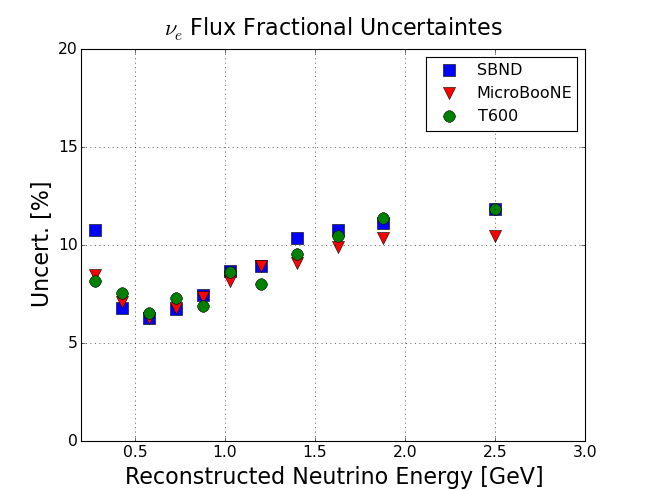
\includegraphics[width=0.75\textwidth]{systematics_figures/matrixFile_nue_ND_100m_uB_T600_onaxis_flux_6_ecalo2_nu_vePhot0.05_gap3_fracUncert}
    \caption[Fractional Flux Uncertainties]{The systematic uncertainties in the \nue appearance event rates for the SBN program, coming from uncertainties in the neutrino flux.  This includes flux-based uncertainties for both the \nue component, from the \nue flux, and the \numu misidentified component of the background.}
   \label{fig:sys_flux_uncert_fracUncert}
\end{figure}

\begin{figure}[]
    \centering
    \includegraphics[width=0.5\textwidth]{systematics_figures/matrixFile_nue_ND_100m_uB_T600_onaxis_flux_6_ecalo2_nu_vePhot0.05_gap3_fracMatHist}
    \caption[Flux Fractional Covariance Matrix]{The fractional covariance matrix for the flux uncertainties.  The uncertainties are highest in the tails of each detector's distributions.}
   \label{fig:syst_flux_fracmatrix}
\end{figure}
\begin{figure}[]
    \centering
    \includegraphics[width=0.5\textwidth]{systematics_figures/matrixFile_nue_ND_100m_uB_T600_onaxis_flux_6_ecalo2_nu_vePhot0.05_gap3_corrMatHist}
    \caption[Flux Correlation Matrix]{The correlation matrix for the flux uncertainties. The uncertainties are highly correlated across the three detectors, which is essential to achieving a strong cancellation between detectors. }
   \label{fig:syst_flux_corrmatrix}
\end{figure}



\section{Uncertainties from Neutrino Interactions}

After the flux uncertainty, the largest remaining uncertainty in a multidetector analysis is the uncertainty coming from neutrino interactions.  In particular, the flux and cross section uncertainties combine to form the overall normalization uncertainty on the event rates.

The use of the covariance method to compute a $\chi^2$ would be incorrect if the major normalization uncertainties were not all accounted for.  To address this, the systematic uncertainties from the neutrino interactions are also addressed with a covariance matrix.  As the simulation uses GENIE \cite{Andreopoulos:2009rq} to simulate neutrino interactions within argon, the same event generator was used to calculate the systematic uncertainties for cross sections.

At it's core, GENIE is a cross section calculator for neutrino interactions.  It models known interactions by computing cross section splines for a reaction between a specific flavor of neutrino and a nuclear target.  These splines are slow to create, and need to be comprehensive to have accurate results in the simulation.  At runtime, however, GENIE doesn't recompute cross sections for a particular neutrino onto a target if it is already computed, it just accesses the spline for the information.

All of the cross sections that GENIE computes are based on theory or fits to experimental data, and hence the parameters used (in the theory or fits) have some systematic uncertainty associated with them.  By varying these parameters according to their 1 $\sigma$ uncertainty, and recomputing the cross section, a weight can be applied to the event as described above in section Section ~\ref{sec:multi_weight}.

The GENIE framework provides a model for consistent variations of systematic uncertainties.  When, for example, a total cross section is constrained by data and a variation is requested on a subset of that total cross section, the other subsets are adjusted to compensate.  This gives a consistent ``Universe'' across all neutrino interactions when the underlying parameters are adjusted.

Table~\ref{tab:genie_xsec_params} shows the parameters that were varied in the GENIE cross section calculator for this analysis.  In each ``Universe,'' every parameter was varied within it's 1 $\sigma$ Gaussian distribution and the weights for each interaction were calculated, for a total of 250 universes.  Figure~\ref{fig:sys_xsec_uncert_fracUncert} shows the level of uncertainty in the detector's final \nue event rates arising from the cross section uncertainties.  This is, without a multi detector analysis, a very large source of uncertainty on the interaction rates.

{
\renewcommand{\arraystretch}{1.5}
\begin{table}[tb]
  \caption[Genie Cross Section Variations]{Genie Cross Section Variations and their nominal uncertainty, from \cite{Andreopoulos:2015wxa}}
  \label{tab:genie_xsec_params}
  \centering

  \begin{tabular}{l|lc}
  \hline

  \hline
  \textbf{Parameter} & \textbf{Description} & \textbf{Nominal Variation} \\
  \hline
     $M_A^{CCQE}$ & Axial Mass for CC Quasi-Elastic & -15\% +25\%  \\
     $M_A^{CCRES}$ & Axial Mass for CC Resonance Production & $\pm$20\%  \\
     $M_A^{NCRES}$ & Axial Mass for NC Resonance Production & $\pm$20\%  \\
     $R_{bkg}^{\nu p, CC 1 \pi}$& Non-resonance Background in CC 1 $\pi$ production & $\pm$ 50\% \\
     $R_{bkg}^{\nu p, CC 2 \pi}$& Non-resonance Background in CC 2 $\pi$ production & $\pm$ 50\% \\
     $R_{bkg}^{\nu n, CC 1 \pi}$& Non-resonance Background in CC 1 $\pi$ production & $\pm$ 50\% \\
     $R_{bkg}^{\nu n, CC 2 \pi}$& Non-resonance Background in CC 2 $\pi$ production & $\pm$ 50\% \\
     $R_{bkg}^{\nu p, NC 1 \pi}$& Non-resonance Background in NC 1 $\pi$ production & $\pm$ 50\% \\
     $R_{bkg}^{\nu p, NC 2 \pi}$& Non-resonance Background in NC 2 $\pi$ production & $\pm$ 50\% \\
     $R_{bkg}^{\nu n, NC 1 \pi}$& Non-resonance Background in NC 1 $\pi$ production & $\pm$ 50\% \\
     $R_{bkg}^{\nu n, NC 2 \pi}$& Non-resonance Background in NC 2 $\pi$ production & $\pm$ 50\% \\
     % DIS Nucl. Model & & \\
  \hline

  \hline
  \end{tabular}
\end{table}
}


\begin{figure}[h]
    \centering
    \includegraphics[width=0.75\textwidth]{systematics_figures/matrixFile_nue_ND_100m_uB_T600_onaxis_xsec_0_ecalo2_nu_vePhot0.05_gap3_fracUncert}
    \caption[\nue Cross Section Uncertainties]{Fractional uncertainties at each detector in the \nue analysis due to neutrino interaction uncertainties.}
   \label{fig:sys_xsec_uncert_fracUncert}
\end{figure}

\begin{figure}[h]
    \centering
    \includegraphics[width=0.5\textwidth]{systematics_figures/matrixFile_nue_ND_100m_uB_T600_onaxis_xsec_0_ecalo2_nu_vePhot0.05_gap3_fracMatHist}
    \caption[\nue Cross Section Fractional Covariance Matrix]{The fractional covariance matrix from the cross section uncertainties.}
   \label{fig:syst_xsec_fracmatrix}
\end{figure}

\begin{figure}[h]
    \centering
    \includegraphics[width=0.5\textwidth]{systematics_figures/matrixFile_nue_ND_100m_uB_T600_onaxis_xsec_0_ecalo2_nu_vePhot0.05_gap3_corrMatHist}
    \caption[\nue Cross Section Correlation Matrix]{The correlation matrix for the cross section uncertainties in the \nue analysis.  As seen by the very high correlation across the analysis bins, the cross section uncertainties are mostly a normalization uncertainty and not a shape uncertainty.}
   \label{fig:syst_xsec_corrmatrix}
\end{figure}


As seen in Figure~\ref{fig:syst_xsec_corrmatrix}, the cross section uncertainties across the detectors (and amongst the analysis bins within a detector) are highly correlated.  The even correlation indicates that the uncertainty is largely a normalization uncertainty, and not indicative of a different uncertainty in the energy dependence of the cross section, for example.  The only regions where the correlation is not as strong is the lowest energy bin to the higher energy bins in each detector.  Since the lowest energy bin has the highest rate of misidentified events, coming from Neutral Current pion producing interactions, it is sensible that this bin is less correlated to the rest.

Despite the very high correlation of cross section uncertainties, there are two caveats to this part of the study of systematic uncertainties in the SBN Program.  First, the uncertainties studied did not include final state interaction variations.  Because this is a Charged Current inclusive analysis, the final state interaction uncertainties should have minimal impact on the final result.  Any analysis that uses an exclusive channel, such as CC \nue 0 pion, would need a very careful study of the neutrino generator model and it's included uncertainties.

Second, the GENIE neutrino generator includes a package for systematic uncertainty study, however this list of channels studied is not expected to be 100\% comprehensive.  Instead, it serves to validate and quantify the level of correlation between the SBN detectors.

Despite these caveats, the conclusion of the cross section analysis is quite strong: whatever systematic uncertainties arise from neutrino interactions, they are very strongly correlated across the 3 detectors.  The quantification of that correlation is encoded in the covariance matrix, Figure~\ref{fig:syst_xsec_fracmatrix}.

\section{Residual Systematic Uncertainties}

After considering the flux and cross section uncertainties in detail, it is reasonable to ask what is the residual systematic uncertainty on a \nue appearance measurement in the SBN Program.

There are two types of uncertainties that are not studied in great detail yet, correlated and uncorrelated.  Some examples of correlated uncertainties that will be studied in the future, before the final analysis, are

\begin{itemize}
  \item {\bf Reconstruction Efficiencies} - the three detectors of the SBN Program will all use the same suite of reconstruction tools to build their event rates.  The efficiency will not be perfect, as no set of particle reconstruction software ever is, however the systematic biases introduced by the reconstruction will be correctable through Monte Carlo and well correlated between the detectors.  For the study shown here, reconstruction efficiencies are assumed to be the same across all three detectors.
  \item{\bf Cosmogenic Backgrounds} - the cosmogenic background, which occurs when a cosmic particle produces an interaction that is mistaken for an electron neutrino, will be mostly correlated between the three detectors.  There is some variance in the building geometries, such as overburdens and cosmic tagging systems (muon detectors external to the cryostat), however the basic cosmic flux at all three detectors will be correlated.  Further, the cosmogenic background can be measured with nearly arbitrary precision with off-beam spills.  That is, since the neutrino beams are pulsed there are clear samples of data with {\bf no} neutrinos, which can be used to measure the amount of cosmogenic misidentification as electron neutrinos.  Under this assumption, the covariance matrix for the cosmic sample is the statistical uncertainty of the cosmic misidentification in the accepted event samples.

\end{itemize}

On the other hand, residual uncorrelated uncertainties include

\begin{itemize}
  \item {\bf Detector Effects} - The three detectors of the SBN Program, while all LArTPCs, are not identical detectors in the same way that Daya Bay is, for example \cite{An:2015qga}.  As described in Section~\ref{sec:sbn_detectors}, the three detectors have some differences.  \uboone is a single drift detector, while \icarus and \sbnd are dual drift TPCs with a cathode in the middle.  Further, the fiducial volumes of the detectors are different, and the ability to contain neutral particles and electromagnetic particles is different due to the different shape of the detectors.
  \item{\bf ``Dirt'' Backgrounds} - the backgrounds produced by the beam but externally to the detector will, to first order, be uncorrelated between detectors.  The overall rate will fluctuate up or down with the neutrino flux, however the complexity of the surrounding material of the detectors makes the evaluation difficult.  Therefore, to be conservative, a 15\% uncertainty is applied to the ``Dirt'' backgrounds at each detector.  This is assumed to be fully correlated within each detector's analysis bins, but uncorrelated across detectors.
\end{itemize}

Before a final analysis is released, these systematics uncertainties must be carefully addressed.

\section{Sensitivity to Anomalous \nue Appearance at the SBN Program}

To evaluate the expect sensitivity of the SBN Program, the above covariance matrices are used as shown in Equation~\ref{eq:tot_cov_mat}.  The $\chi^2$ measure of sensitivity is computed as in Equation~\ref{eq:chi_sq}.  The final sensitivity to \nue is shown in Figure~\ref{fig:sbn_final_sensitivity}.  As an alternative view to this sensitivity, the quoted sensitivity in Figure~\ref{fig:sbn_alt_sensitivity} shows the $\sqrt{\chi^2}$ of calculated along the left edge of the LSND 90\% confidence region.


\begin{figure}[tb]
  \centering
  \includegraphics[width=0.75\textwidth]{systematics_figures/{ND_100m_uB_T600_onaxis_nue_appearance_ecalo2_nu_vePhot0.05_gap3_lessCosmics_xsec_0_flux_6_dirt_cos_sensPlot.pdf}}
  \caption[SBN Sensitivity]{The SBN Program's quoted sensitivity, under all the assumptions shown above. At the best fit points from \cite{Kopp:2013vaa} and \cite{Giunti:2011gz}, the significance is well above 5 $\sigma$.}
  \label{fig:sbn_final_sensitivity}
\end{figure}



\begin{figure}[tb]
  \centering
  \includegraphics[width=\textwidth]{systematics_figures/{nominalSBNSens.pdf}}
  \caption[SBN Sensitivity Along LSND Edge]{The SBN Sensitivity along the lower edge of the LSND 90\% confidence allowed region.  Because of the low $\text{sin}^22\theta$ values along the LSND regions left edge, this is a region with a very small and difficult to measure signal.  Therefore, it is a good parameter space with which to measure the SBN Sensitivity.}
  \label{fig:sbn_alt_sensitivity}
\end{figure}

\chapter{Electron Neutrino Interactions and Data Reconstruction}

\section{Interactions in Argon}

\section{Detector Signatures}

\section{Reconstructing Electron Neutrinos in \lartpcs}


\chapter{Reconstruction and Analysis of Electron Neutrinos in \argoneut }

\section{Identifying and Reconstruction Electromagnetic Showers}

\section{Electron/Photon Separation}
\label{sec:e_gamma_sep}
\subsection{dE/dx and Topological}
\subsection{Efficiency of rejection of photons and systematic error}

\section{Reconstruction Efficiency}
\subsection{systematics}

\chapter{\label{chp:nue_xsec} Electron Neutrino Cross Section on Argon}

\section{Measurement of Neutrino Cross Sections}

\section{Electron Neutrino Flux at \argoneut}

\section{Cross Section Results}

\section{Systematic Uncertainties} 

\chapter{Conclusions} 

% Add additional \chapter{}s as necessary.

% use \cite{} to cite a reference in your bibliography file.
% use \ref{} to reference a \label{} from an equation, figure, or table.

% for sets of equations use align or gather:
%\begin{align}
%\end{align}

% for long equations, use multline.

% for figures:
%\begin{figure}[ht]
%\centering
%\includegraphics[width=.45\textwidth]{name_of_figure.eps}
%\caption{A caption! \label{a_figure}}
%\end{figure}

% for tables:
%\begin{table}
%\begin{tabular}{c|c|c}
% 1 & 2 & 3 \\
%\hline
%\end{tabular}
%\caption{Another caption! \label{a_table}}
%\end{table}


% Only call appendix once, here.
\appendix

\chapter{Stuff}
If you need an appendix, it will go here.

\begin{align}
a^n + b^n &\ne c^n \\
n &> 2
\end{align}

\chapter{More stuff}
A second appendix. Look at you, you over achiever.





% Any chapters such as End Notes go after this.
\backmatter


\bibliography{references}
% for your own sake, use a bibtex file, so all of the numbering of references will be done
% automatically.



\end{document}
